\documentclass[11pt,dvipsnames]{article}
%\documentclass[12pt,usenames,dvipsnames]{article}
\usepackage{titling}
\newcommand{\subtitle}[1]{%
  \posttitle{%
    \par\end{center}
    \begin{center}\large#1\end{center}
    \vskip0.5em}%
}
\usepackage[dvipsnames]{xcolor}
\usepackage{setspace}
%\doublespacing
%\usepackage[longnamesfirst]{natbib}
\usepackage{natbib}
%\usepackage[margin=1.2cm]{geometry}
\usepackage[margin=2.5cm]{geometry}
\onehalfspacing
%\usepackage{fancyhdr}% http://ctan.org/pkg/fancyhdr
%\fancyhead{}% Clear all headers
%\fancyfoot{}% Clear all footers
%\fancyfoot[L]{Filip Stan\v{e}k}% Place "My Name" in Center of header
%\fancyfoot[R]{\thepage}% Page number in Right footer
%\renewcommand{\headrulewidth}{0pt}% Remove header rule
%%\renewcommand{\footrulewidth}{0pt}% Remove footer rule
%\pagestyle{fancy}% Set page style to "fancy"
\usepackage{hyperref}
\usepackage[justification=centering]{caption}
\newcommand\fnote[1]{\captionsetup{font=footnotesize}\caption*{#1}}
\usepackage{graphicx}
\providecommand{\keywords}[1]{\textbf{Key Words:} #1}
\usepackage{amsmath}
\usepackage{amsfonts}
\usepackage{bbm}
\usepackage{enumitem}
\usepackage{tikz}
\usetikzlibrary{matrix}
\usetikzlibrary{matrix,positioning}
\usepackage{subcaption} 
\usetikzlibrary{backgrounds}
\usepackage{makecell}
\tikzset{
diagonal fill/.style 2 args={fill=#2, path picture={%
\fill[#1] (path picture bounding box.south west) -|
                         (path picture bounding box.north east) -- cycle;}},
reversed diagonal fill/.style 2 args={fill=#2, path picture={
\fill[#1] (path picture bounding box.north west) |- 
                         (path picture bounding box.south east) -- cycle;}}
}
\newtheorem{proposition}{Proposition}
\newtheorem{assumption}{Assumption}
\newtheorem{proof}{Proof of Proposition}
\newtheorem{lemma}{Lemma}
\newtheorem{algorithm}{Algorithm}
\newtheorem{estimator}{Estimator}
\usepackage{caption}
\captionsetup{width=15cm}
\captionsetup{font=footnotesize}
\DeclareMathOperator{\vect}{vec}
\DeclareMathOperator{\omitt}{omit}
\DeclareMathOperator{\cardt}{card}
\DeclareMathOperator{\NAT}{NA}

\usepackage{multirow}
\usepackage{subcaption}
\usepackage{tabularx}
\usepackage[affil-it]{authblk}

\usepackage{pgfplotstable}
\pgfplotsset{compat=1.17}
\usepackage{booktabs}
\usepackage{subcaption}

\usepackage[section]{placeins}
\usepackage{xurl}

\newcommand{\splitatcommas}[1]{%
  \begingroup
  \begingroup\lccode`~=`, \lowercase{\endgroup
    \edef~{\mathchar\the\mathcode`, \penalty0 \noexpand\hspace{0pt plus 1em}}%
  }\mathcode`,="8000 #1%
  \endgroup
}

\pgfplotstableset{
    highlight/.append style={
        postproc cell content/.append code={
                %\pgfkeysalso{@cell content=\textbf{##1}}%
                \pgfkeysalso{@cell content/.add={$\bf}{$}}%
        },
    },
    highlightrow/.append style={
        postproc cell content/.append code={
           \count0=\pgfplotstablerow
            \advance\count0 by1
            \ifnum\count0=#1
            %\pgfkeysalso{@cell content/.add={$\bf}{$}}%
               \pgfkeysalso{@cell content=\textbf{##1}}%
            \fi
        },
    },
    highlightcol/.append style={
        postproc cell content/.append code={
           \count0=\pgfplotstablecol
            \advance\count0 by1
            \ifnum\count0=#1
            \pgfkeysalso{@cell content/.add={$\bf}{$}}%
               %\pgfkeysalso{@cell content=\textbf{##1}}%
            \fi
        },
    },
}

\usepackage[toc,page]{appendix}
\newcommand{\possessivecite}[1]{\citeauthor{#1}'s (\citeyear{#1})}

\begin{document}
\title{
\Large{Optimal Out-of-Sample Forecast Evaluation Under Stationarity}}
% \author{$  $}
\author{
  Filip Stan\v{e}k\thanks{
  % \texttt{redacted}\thanks{
  E-mail: \texttt{filip.stanek@cerge-ei.cz}.
  % E-mail:\texttt{redacted}.
  % Financial support from Grantová agentura UK under grant 264120 is gratefully acknowledged.
  % Financial support from Grantová agentura UK under grant \texttt{redacted} is gratefully acknowledged.
  % Furthermore, I'm thankful to prof. Stanislav Anatolyev for numerous valuable suggestions and to two anonymous referees, whose insightful feedback greatly enhanced clarity of the manuscript and helped strengthen the results.
  % Furthermore, I'm thankful to \texttt{redacted} for numerous valuable suggestions and to two anonymous referees, whose insightful feedback greatly enhanced clarity of the manuscript and helped to strengthen the results.
}
}

%\affil{$  $}
\affil{
  CERGE-EI\thanks{CERGE-EI, a joint workplace of Charles University and the Economics Institute of the Czech Academy of Sciences, Politickych veznu 7, 111 21 Prague, Czech Republic.}
  % \texttt{redacted}
}


\maketitle
\begin{abstract}
It is a common practice to split a time series into an in-sample and pseudo out-of-sample segments and estimate the out-of-sample loss for a given statistical model by evaluating forecasting performance over the pseudo out-of-sample segment. We propose an alternative estimator of the out-of-sample loss, which, contrary to the conventional wisdom, utilizes criteria measured both in- and out-of-sample via a carefully constructed system of affine weights. We prove that, provided that the time series is stationary, the proposed estimator is the best linear unbiased estimator of the out-of-sample loss, and outperforms the conventional estimator in terms of sampling variability. Application of the optimal estimator to Diebold-Mariano type tests of predictive ability leads to a substantial power gain without increasing finite sample size distortions. An extensive evaluation on real world time series from the M4 forecasting competition confirms superiority of the proposed estimator, and also demonstrates substantial robustness to violations of the underlying assumption of stationarity.
\end{abstract}
\bigskip 
\bigskip 
\bigskip 
\textbf{Keywords:} Loss Estimation, Forecast Evaluation, Cross-Validation, Model Selection\\
\textbf{JEL classification codes:} C22, C52, C53
\thispagestyle{empty}
\newpage 

\section{Introduction}

In the field of time series forecasting, researchers are typically concerned with the expected performance of a particular statistical model on yet unseen data, the so called out-of-sample loss. It is used to assess whether a proposed model statistically significantly outperforms an already established benchmark model. Likewise, in practical forecasting tasks, the out-of-sample loss is frequently used to select a model that is likely to deliver the best forecasting performance from a set of competing models. 

Out-of-sample loss is defined as the expected value of a contrast function that measures the discrepancy between the prediction and the observed value (e.g., the expected value of squared error). Thus, it is by definition unknown and needs to be estimated. This is typically achieved by excluding the most recent segment of the observed time series from the estimation and performing a sequence of predictions for these observations instead, essentially mimicking the process of actual out-of-sample forecasting.\footnote{There is another class of evaluation schemes that do not respect the temporal ordering of the data and perform out-of-sample evaluation not dissimilar to the canonical cross-validation for independent processes, see e.g., \citet{burmanCrossvalidatoryMethodDependent1994}, \citet{racineConsistentCrossvalidatoryModelselection2000}, and \citet{bergmeirNoteValidityCrossvalidation2018}. However, these are not as widely used in practice and hence are not considered in this article.} The estimate of the out-of-sample loss is then obtained simply by averaging the precision of individual predictions as measured by the contrast function, i.e., the so called empirical contrasts (e.g. squared errors). While there are many such pseudo out-of-sample evaluation schemes \citep[for a survey, see][]{tashmanOutofsampleTestsForecasting2000}, we restrict our attention to two prominent variants; the rolling scheme and the fixed scheme. When performing an evaluation under the rolling scheme, the model is repeatedly estimated on a rolling window of a fixed length and predictions are made for the subsequent observations. In the fixed scheme, the model is estimated only once on the first segment of the data and is then used to predict all remaining observations \citep[see e.g.][]{clarkChapter20Advances2013}.

A common drawback of all such pseudo out-of-sample evaluation schemes and corresponding estimators is the relatively high sampling variance, as the estimate is computed based on only a relatively few most recent observations reserved for the pseudo out-of-sample evaluation \citep[][]{bergmeirUseCrossvalidationTime2012,bergmeirUsefulnessCrossvalidationDirectional2014,schnaubeltComparisonMachineLearning2019,cerqueiraEvaluatingTimeSeries2020}. Moreover, this issue of scarcity of pseudo out-of-sample observations and consequently of high sampling variance is not limited to situations with few observations, but also afflicts longer time series. This is because there is an inevitable trade-off between the size of the data-sets designated to be in-sample and pseudo out-of-sample. The former allows for a more faithful approximation of the loss when the whole data-set is used for estimation, whilst the latter allows for more precise estimation of the loss \citep[see][]{arlotSurveyCrossvalidationProcedures2010}. 

To alleviate this issue, we propose an alternative estimator of the out-of-sample loss that utilizes in-sample performance to aid the estimation of the out-of-sample loss, a practice often considered taboo in the forecasting community. In particular, we use in-sample empirical contrasts to partially eliminate the idiosyncratic noise present in observations designated for the out-of-sample evaluation, via a carefully constructed system of optimal affine weights. We prove that, under stationarity, the proposed estimator of the out-of-sample loss is optimal in terms of the sampling variance within the class of unbiased linear estimators, to which the conventional estimator also belongs. The proposed estimator hence offers a lower sampling variance relative to the conventional estimator, all without introducing any bias. In turn, this allows for a finer assessment of forecasting ability, more powerful inference about predictive ability, and more precise model selection.

The proposed optimal estimator is obtained by finding weights that minimize the sampling variance, subject to constraints that guarantee unbiasedness. Importantly, both in- and out-of-sample contrasts can be included with non-zero weights, and weights are allowed to be negative, unlike for the conventional estimator, which simply places equal positive weights only on out-of-sample contrasts. In practice, this translates to assigning negative weights to in-sample empirical contrasts that are positively correlated with out-of-sample empirical contrasts, and positive weights to in-sample empirical contrasts that are uncorrelated with out-of-sample empirical contrasts. At the same time, sums of weights of ex-ante identical in-sample contrasts are equal to zero, which ensures that the inclusion of in-sample contrasts does not alter the expected value of the estimator, and hence does not introduce bias. From a more general standpoint, the possibility to reduce the sampling variance arises because time series out-of-sample evaluation schemes are inherently unbalanced in the sense of \citet{shaoLinearModelSelection1993}. That is, these schemes generally do not treat observations equally in terms of in-/out-of-sample usage. The proposed optimal weighting partially rectifies this unbalanced design.

Aside from the optimal estimator itself, we also propose modifications of the canonical Diebold-Mariano test \citep{dieboldComparingPredictiveAccuracy1995} and of the sub-sampling test of equal predictive ability \citep{zhuCanTwoForecasts2020,ibragimovTStatisticBasedCorrelation2010}. Both modified tests leverage the proposed optimal weighting for estimation of the loss differential. We show that these tests are asymptotically valid and demonstrate that they exhibit a substantially higher power in detecting deviations from the null hypothesis of equal predictive ability relative to their respective benchmarks.

Finally, to assess the real-life applicability and the robustness of the proposed estimator, we perform an extensive evaluation on 100,000 time series from the M4 forecasting competition  \citep{makridakisM4Competition1002020} ranging from yearly to hourly frequency. The proposed estimator delivers more than a $ 10\%$ reduction in the mean squared error relative to the conventional estimator when tasked with predicting the incurred loss on the test segments of time series. Moreover, when selecting the model by comparing estimated losses, the proposed optimal estimator is more likely to select the best performing model and delivers a smaller overall incurred loss. Importantly, we take no special care to ensure that the time series are stationary in this evaluation. In fact, most series in the M4 competition do exhibit either some trend, seasonality, or both. Despite this adverse setting, the proposed estimator still substantially outperforms the conventional estimator, exhibiting a remarkable robustness to the violation of the underlying assumption of stationarity. This clearly demonstrates that the theoretical superiority of the proposed estimator does extend to actual forecasting applications, even with all the difficulties that forecasting real time series entails.

Section \ref{ConventionalEstimator} introduces the statistical framework and provides formal definitions of out-of-sample evaluation schemes and corresponding estimators. Section \ref{Estimator} introduces the proposed estimator of the out-of-sample loss, proves its optimality, and demonstrates its efficiency gains in a simulated environment. Section \ref{TestingFiniteSamplePredictiveAbility} introduces modified tests of equal out-of-sample predictive ability that utilize the optimal estimator, and demonstrates their power advantage relative to benchmarks. Section \ref{EmpiricalEvaluation} compares the performance of the conventional estimator and the proposed optimal estimator on real world time series from the M4 forecasting competition. Section \ref{Conclusions} concludes. Appendices \ref{appendix:Proofs}, \ref{appendix:Estimators}, \ref{appendix:Algorithms}, and \ref{appendix:Additional} contain proofs, estimators, algorithms, and auxiliary results, respectively. A ready-to-use implementation of the estimator and tests is provided as an R software package \textit{ACV}\footnote{Available at: \url{https://CRAN.R-project.org/package=ACV}.}.
%\footnote{Available at: \textit{redacted for peer review}.}
%\footnote{Available at: \url{https://github.com/stanek-fi/ACV}.}

\section{Conventional Estimator of the Loss}\label{ConventionalEstimator}

% Consider a $ d $-variate sequence $ \left\lbrace X_{t} \right\rbrace_{1}^{T} \in \left( \mathbb{R}^{d}\right) ^{T} $ from a stationary random process $ X_{t} $ for a given $ T \in \mathbb{N}$.
% Following the notation of \citet{arlotSurveyCrossvalidationProcedures2010}, a statistical model $ \mathcal{M} = \lbrace s,\, \widehat{\theta} \rbrace $ is composed of two functions; the estimator $ \widehat{\theta}\left( \left\lbrace X_{t} \right\rbrace_{1}^{m}\right)  $ generating estimated parameters and the forecasting function $ s\left( \left\lbrace X_{t} \right\rbrace_{1}^{k};\, \theta\right)  $, which predicts the upcoming value of the process based on past values and parameters $ \theta $.\footnote{To facilitate the exposition, we take the liberty of representing the model as a prediction and estimation function pair $ \mathcal{M} = \lbrace s,\, \widehat{\theta} \rbrace $ rather than a single function $ \mathcal{A} $ representing a statistical algorithm as in \citet{arlotSurveyCrossvalidationProcedures2010}, hence focusing on parametric models.
% All results can nonetheless be extended to non-parametric models by using the identity $ \mathcal{A}\left( \left\lbrace X_{t} \right\rbrace_{1}^{m}\right)\left( \left\lbrace X_{t} \right\rbrace_{j-k-\tau+1}^{j-\tau} \right)  =s\left(\left\lbrace X_{t} \right\rbrace_{j-k-\tau+1}^{j-\tau} ;\,\widehat{\theta}\left( \left\lbrace X_{t} \right\rbrace_{1}^{m} \right) \right)   $.} In particular, $ \widehat{\theta}:\cup_{m \in \mathbb{N}} \left( \mathbb{R}^{d}\right)^{m}\rightarrow \Theta $ where $ \Theta $ is a parameter space and $ m $ is the number of observations used for the estimation.
% Predictions about the $ \tau $-th upcoming value of the process are made via function $ s:\lbrace \left( \mathbb{R}^{d}\right)^{k};\, \Theta \rbrace \rightarrow \Psi $, where $ \tau $ is the forecasting horizon, $ \Psi $ represent the space of all such possible predictions, and $ k $ is the number of past values of the process used to predict the $ \tau $-th upcoming value.
% To assess the quality of a model $ \mathcal{M}  $, we use a contrast function $ \gamma: \lbrace  \mathbb{R}^{d},\, \Psi \rbrace  \rightarrow \mathbb{R}$ that measures the discrepancy between a prediction $ \psi \in \Psi $ and the actual realization of the process.

% This rather general framework allows us to simultaneously consider many typical applications encountered in time series forecasting.
% For example, in the case of uni-variate step ahead mean forecasting,  $ \tau =1$, and the space of possible predictions $ \Psi = \mathbb{R} $.
% A model $ \mathcal{M} $ could be AR($ k $) with the corresponding least square estimator, in which case the parameter space $ \Theta = \mathbb{R}^{k}$ and prediction $ \psi = s(\left\lbrace X_{t} \right\rbrace_{1}^{k};\, \widehat{\theta}) = \sum_{1}^{k} X_{k} \widehat{\theta}_{k}$ where $ \widehat{\theta} $ is an OLS estimator.
% A contrast function is typically a squared error, and hence $ \gamma\left(X_{k+1},\, \psi\right)=\left( X_{k+1} - \psi \right)^{2} = \left( X_{k+1} - \sum_{1}^{k} X_{k} \widehat{\theta}_{k} \right)^{2}$. 
% In the case of univariate conditional density forecasting, a model $ \mathcal{M} $ could be a class of densities and a corresponding estimator $ \widehat{\theta} $ for its parameters, set $ \Psi $ is a space of density functions and  $ \psi(q) = s\left( \left\lbrace X_{t} \right\rbrace_{1}^{k};\, \widehat{\theta}\right) \left( q\right)  = \widehat{f}\left( q| \left\lbrace X_{t} \right\rbrace_{1}^{k}; \widehat{\theta} \right)$ is the predicted density at point $ q $.
% One may take $ \gamma\left(X_{k+\tau}, \psi\right) = -ln\left(\psi\left( X_{k+\tau}\right) \right) = -ln\left( \widehat{f}\left( X_{k+\tau}| \left\lbrace X_{t} \right\rbrace_{1}^{k};\, \widehat{\theta} \right) \right)$ to obtain the Kullback-Leibler divergence \citep{kullbackInformationSufficiency1951} as a measure of precision of $ \psi $.

We follow the notation of \citet{arlotSurveyCrossvalidationProcedures2010}.
Consider a sequence $ \left\lbrace X_{t} \right\rbrace_{1}^{T} \in \mathbb{R}^{T} $ from a stationary random process $ X_{t} $ for a given $ T \in \mathbb{N}$.
A statistical model $ \mathcal{M} = \lbrace s,\, \widehat{\theta} \rbrace $ is composed of two functions.
The estimator $ \widehat{\theta}:\cup_{m \in \mathbb{N}} \mathbb{R}^{m}\rightarrow \Theta $, which takes sequence $\left\lbrace X_{t} \right\rbrace_{1}^{m}$ of length $m$ and outputs model parameters $\theta$ belonging to the parameter space $\Theta$,
and the forecasting function $ s:\lbrace  \mathbb{R}^{k};\, \Theta \rbrace \rightarrow \mathbb{R}$, which predicts the observation $X_{k+\tau}$ based on most recent observations $\left\lbrace X_{t} \right\rbrace_{t=1}^{k}$ where $k$ is the memory of the model and $\tau$ is the forecast horizon.\footnote{
  To facilitate the exposition, we take the liberty of representing the model as a prediction and estimation function pair $ \mathcal{M} = \lbrace s,\, \widehat{\theta} \rbrace $ rather than a single function $ \mathcal{A} $ representing a statistical algorithm as in \citet{arlotSurveyCrossvalidationProcedures2010}, hence focusing on parametric models.
  All results can nonetheless be extended to non-parametric models by using the identity $ \mathcal{A}\big( \left\lbrace X_{t} \right\rbrace_{1}^{m}\big)\big( \lbrace X_{t} \rbrace_{j-k-\tau+1}^{j-\tau} \big)  =s\big(\lbrace X_{t} \rbrace_{j-k-\tau+1}^{j-\tau} ;\,\widehat{\theta}\big( \left\lbrace X_{t} \right\rbrace_{1}^{m} \big) \big)   $.
}
To assess the quality of a model $ \mathcal{M}  $, we use a contrast function $ \gamma: \lbrace  \mathbb{R},\, \mathbb{R} \rbrace  \rightarrow \mathbb{R}$ that measures the discrepancy between a prediction $\hat{X}_{k+\tau} = s(\left\lbrace X_{t} \right\rbrace_{t=1}^{k},\, \theta) $ and the actual realization of the process $X_{k+\tau}$. 
For instance, a simple AR($ k $) model would correspond to  $ \widehat{X}_{k+1} = s(\left\lbrace X_{t} \right\rbrace_{1}^{k};\, \widehat{\theta}) = \sum_{1}^{k} X_{k} \widehat{\theta}_{k}$ where $ \widehat{\theta} $ is the corresponding OLS estimator.
Contrast function is typically a squared error in which case $ \gamma\big(X_{k+1},\, \widehat{X}_{k+1}\big)=\big( X_{k+1} - \widehat{X}_{k+1} \big)^{2} $.\footnote{
  Throughout the text, we focus exclusively on univariate point prediction for the sake of simplicity. 
  The framework can be however readily extended to a general $d$-variate prediction problem by considering $ s:\lbrace \big( \mathbb{R}^{d}\big)^{k};\, \Theta \rbrace \rightarrow \Psi $ and $ \gamma: \lbrace  \mathbb{R}^{d},\, \Psi \rbrace  \rightarrow \mathbb{R}$ where $ \Psi $ represents the space of possible predictions. 
  For instance, in the case of univariate conditional density forecasting, a model $ \mathcal{M} $ is a class of densities with a corresponding estimator $ \widehat{\theta} $ for its parameters, set $ \Psi $ is a space of density functions and  $ \psi(q) = s\big( \lbrace X_{t} \rbrace_{1}^{k};\, \widehat{\theta}\big) \big( q\big)  = \widehat{f}\big( q| \lbrace X_{t} \rbrace_{1}^{k}; \widehat{\theta} \big)$ is the predicted density at point $ q $.
  One may take $ \gamma\big(X_{k+\tau}, \psi\big) = -\ln\big(\psi\big( X_{k+\tau}\big) \big) = -\ln\big( \widehat{f}\big( X_{k+\tau}| \lbrace X_{t} \rbrace_{1}^{k};\, \widehat{\theta} \big) \big)$ to obtain the Kullback-Leibler divergence \citep{kullbackInformationSufficiency1951} as a measure of precision.
}

Finally, let us denote the loss of model $ \mathcal{M}=\lbrace s,\, \widehat{\theta} \rbrace $ when estimated on a sequence of length $ m $ and when faced with forecasting the period $ j>m $  using observations $ \left\lbrace X_{t} \right\rbrace_{j-k-\tau+1}^{j-\tau} $ as
\begin{equation}
\mathcal{L}_{j}^{m}\left(\mathcal{M} \right)=\mathbb{E}\left[ \gamma\left( X_{j}, s\left(\left\lbrace X_{t} \right\rbrace_{j-k-\tau+1}^{j-\tau}; \widehat{\theta}\left(  \left\lbrace X_{t} \right\rbrace_{1}^{m} \right)\right)   \right) \right]. 
\end{equation}
Note that the expectation is taken over the whole segment $ \left\lbrace X_{t} \right\rbrace_{1}^{j} $, i.e., both the forecasted observation $ X_{j} $ and its predecessors, including the estimation window $ \left\lbrace X_{t} \right\rbrace_{1}^{m} $. We are therefore interested in the performance of model $ \mathcal{M} $ rather than that of some particular forecasting function $ s\big(\left\lbrace X_{t} \right\rbrace_{j-k-\tau+1}^{j-\tau}; \theta_{0}\big) $ with fixed $ \theta_{0} \in \Theta $ (i.e., Question 6 from \possessivecite{dietterichApproximateStatisticalTests1998} taxonomy). 

Further, for a ``shifting'' index  $i:\, 0 \leq i \leq T-m$, we also denote the out-of-sample empirical contrast of model $ \mathcal{M} $ when estimated on a sequence $ \left\lbrace X_{t} \right\rbrace_{i+1}^{i+m} $ and evaluated at the $ (i+j) $-th period with $ j>m $ as
\begin{equation}\label{eq:EmpContrastDef} 
l_{j}^{m\,i}\left(\mathcal{M} \right)=\gamma\left( X_{i+j}, s\left(\left\lbrace X_{t} \right\rbrace_{i+j-k-\tau+1}^{i+j-\tau}; \widehat{\theta}\left(  \left\lbrace X_{t} \right\rbrace_{i+1}^{i+m} \right)\right)   \right) . 
\end{equation}
The assumption of stationarity then immediately implies
\begin{equation} \label{eq:EEmpContrast} 
\mathbb{E}\left[l_{j}^{m,\,i}\left(\mathcal{M} \right)\right]=\mathcal{L}_{j}^{m}\left(\mathcal{M} \right).
\end{equation}

In this text, we focus on the pseudo out-of-sample evaluation with step-size $ v $ (see e.g., \citet{callenNeuralNetworkForecasting1996} and \citet{swansonForecastingEconomicTime1997}). The procedure is as follows. The model is estimated on a segment of data of length $ m $ and forecasts are iteratively made on $ v $ consecutive periods for which empirical contrasts are recorded. After that, the estimation window is moved forward by $ v $, and the process is repeated until the end of the sample is reached. The estimate of the out-of-sample loss is then computed simply by averaging all pseudo out-of-sample empirical contrasts incurred. Figure \ref{fig:forwardValidation} provides a diagram of such a procedure. More formally, the estimator is expressed as\footnote{Due to space considerations, we omit $ \mathcal{M} $ from the argument of empirical contrasts, losses, and estimators when it causes no confusion.}
\begin{equation}\label{eq:FVdef} 
\widehat{\mathcal{L}}_{CV}=\dfrac{1}{n}\sum_{i=1}^{n/v}  \sum_{j=1}^{v} l_{m+j}^{m,\,(i-1)v }
\end{equation}
where $ n\equiv T-m $ is the number of observations designated for the pseudo out-of-sample evaluation.\footnote{Throughout this text, we assume that $ n $ is divisible by $ v $, i.e. $ n \bmod v =0 $.} This specification nests the two most common variants of pseudo out-of-sample evaluation. By setting $ v=n $, we obtain the fixed scheme evaluation, which is popular because of its low computational requirements and simplicity. On the other hand, by setting $ v=1 $, we obtain the rolling scheme evaluation, which requires repeated re-estimations, but is presumably more theoretically appealing \citep{swansonForecastingEconomicTime1997}.

\begin{figure}[!htb]
\minipage{0.5\textwidth}%
   \centering
  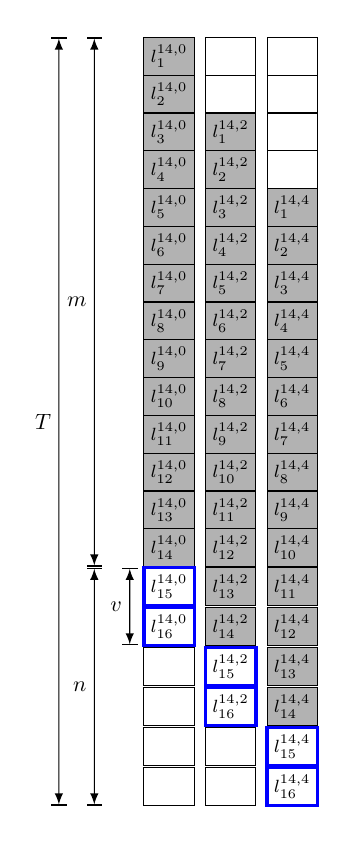
\begin{tikzpicture}[scale=0.9, every node/.style={scale=0.8}]
     \matrix (M) [matrix of nodes,
        nodes={minimum height = 6mm, minimum width =8mm, outer sep=0, anchor=center, draw},
        column 1/.style={nodes={draw=none}},
        column sep=1mm, 
        row sep=-\pgflinewidth, 
        nodes in empty cells,
        i/.style args={#1}{draw, fill=black!30,label={center: \footnotesize #1}},
        ie/.style args={#1}{draw=blue, very thick, fill=black!30,label={center: \footnotesize #1}},
        o/.style args={#1}{draw, fill=blue!0,label={center: \footnotesize #1}},
        oe/.style args={#1}{draw=blue, very thick, fill=blue!0,label={center: \footnotesize #1}}
      ]
      {
        |[i=$ l^{14,0}_{1} $]| & |[o]| & |[o]|  \\
        |[i=$ l^{14,0}_{2} $]| & |[o]| & |[o]|  \\
        |[i=$ l^{14,0}_{3} $]| & |[i=$ l^{14,2}_{1} $]| & |[o]|  \\
        |[i=$ l^{14,0}_{4} $]| & |[i=$ l^{14,2}_{2} $]| & |[o]|   \\ 
        |[i=$ l^{14,0}_{5} $]| & |[i=$ l^{14,2}_{3} $]| & |[i=$ l^{14,4}_{1} $]| \\
        |[i=$ l^{14,0}_{6} $]| & |[i=$ l^{14,2}_{4} $]| & |[i=$ l^{14,4}_{2} $]|  \\
        |[i=$ l^{14,0}_{7} $]| & |[i=$ l^{14,2}_{5} $]| & |[i=$ l^{14,4}_{3} $]|  \\
        |[i=$ l^{14,0}_{8} $]| & |[i=$ l^{14,2}_{6} $]| & |[i=$ l^{14,4}_{4} $]|  \\
        |[i=$ l^{14,0}_{9} $]| & |[i=$ l^{14,2}_{7} $]| & |[i=$ l^{14,4}_{5} $]|  \\
        |[i=$ l^{14,0}_{10} $]| & |[i=$ l^{14,2}_{8} $]| & |[i=$ l^{14,4}_{6} $]| \\
        |[i=$ l^{14,0}_{11} $]| & |[i=$ l^{14,2}_{9} $]| & |[i=$ l^{14,4}_{7} $]|   \\
        |[i=$ l^{14,0}_{12} $]| & |[i=$ l^{14,2}_{10} $]| & |[i=$ l^{14,4}_{8} $]|  \\
        |[i=$ l^{14,0}_{13} $]| & |[i=$ l^{14,2}_{11} $]| & |[i=$ l^{14,4}_{9} $]|  \\
        |[i=$ l^{14,0}_{14} $]| & |[i=$ l^{14,2}_{12} $]| & |[i=$ l^{14,4}_{10} $]|  \\
        |[oe=$ l^{14,0}_{15} $]| & |[i=$ l^{14,2}_{13} $]| & |[i=$ l^{14,4}_{11} $]|  \\
        |[oe=$ l^{14,0}_{16} $]| & |[i=$ l^{14,2}_{14} $]| & |[i=$ l^{14,4}_{12} $]| \\
        |[o]| & |[oe=$ l^{14,2}_{15} $]| & |[i=$ l^{14,4}_{13} $]|  \\
        |[o]| & |[oe=$ l^{14,2}_{16} $]| & |[i=$ l^{14,4}_{14} $]|  \\
        |[o]| & |[o]| & |[oe=$ l^{14,4}_{15} $]| \\
        |[o]| & |[o]| & |[oe=$ l^{14,4}_{16} $]| \\
      };
     \draw ([xshift=-12mm]M-1-1.north west) coordinate (LT) edge[|<->|, >= latex] node[left]{$ T $} ([xshift=-12mm]M-20-1.south west);
     \draw ([xshift=-7mm]M-1-1.north west) coordinate (LT) edge[|<->|, >= latex] node[left]{$ m $} ([xshift=-7mm]M-14-1.south west);
     \draw ([xshift=-7mm]M-15-1.north west) coordinate (LT) edge[|<->|, >= latex] node[left]{$ n $} ([xshift=-7mm]M-20-1.south west);
     \draw ([xshift=-2mm]M-15-1.north west) coordinate (LT) edge[|<->|, >= latex] node[left]{$ v $} ([xshift=-2mm]M-16-1.south west);
  \end{tikzpicture}
    \subcaption{Conventional estimator $ \widehat{\mathcal{L}}_{CV} $. \label{fig:forwardValidation}}
\endminipage\hfill
\minipage{0.5\textwidth}%
   \centering
  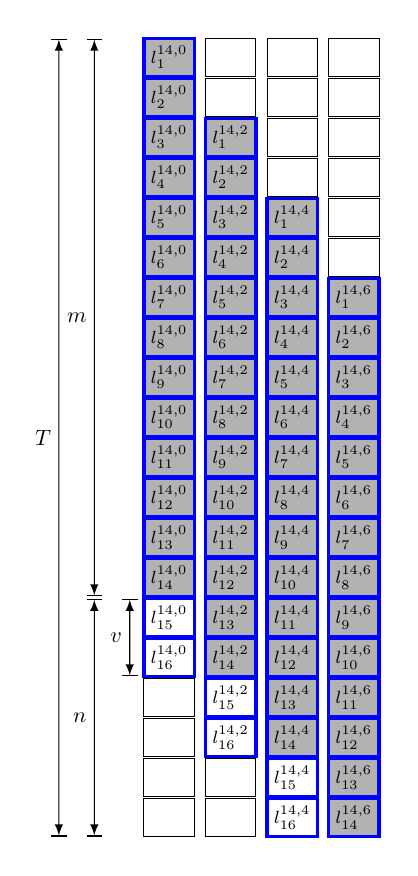
\begin{tikzpicture}[scale=0.9, every node/.style={scale=0.8}]
     \matrix (M) [matrix of nodes,
        nodes={minimum height = 6mm, minimum width =8mm, outer sep=0, anchor=center, draw},
        column 1/.style={nodes={draw=none}},
        column sep=1mm, 
        row sep=-\pgflinewidth, 
        nodes in empty cells,
        i/.style args={#1}{draw, fill=black!30,label={center: \footnotesize #1}},
        ie/.style args={#1}{draw=blue, very thick, fill=black!30,label={center: \footnotesize #1}},
        o/.style args={#1}{draw, fill=blue!0,label={center: \footnotesize #1}},
        oe/.style args={#1}{draw=blue, very thick, fill=blue!0,label={center: \footnotesize #1}}
      ]
      {
        |[ie=$ l^{14,0}_{1} $]| & |[o]| & |[o]| & |[o]| \\
        |[ie=$ l^{14,0}_{2} $]| & |[o]| & |[o]| & |[o]| \\
        |[ie=$ l^{14,0}_{3} $]| & |[ie=$ l^{14,2}_{1} $]| & |[o]| & |[o]| \\
        |[ie=$ l^{14,0}_{4} $]| & |[ie=$ l^{14,2}_{2} $]| & |[o]| & |[o]|  \\ 
        |[ie=$ l^{14,0}_{5} $]| & |[ie=$ l^{14,2}_{3} $]| & |[ie=$ l^{14,4}_{1} $]| & |[o]|  \\
        |[ie=$ l^{14,0}_{6} $]| & |[ie=$ l^{14,2}_{4} $]| & |[ie=$ l^{14,4}_{2} $]| & |[o]| \\
        |[ie=$ l^{14,0}_{7} $]| & |[ie=$ l^{14,2}_{5} $]| & |[ie=$ l^{14,4}_{3} $]| & |[ie=$ l^{14,6}_{1} $]| \\
        |[ie=$ l^{14,0}_{8} $]| & |[ie=$ l^{14,2}_{6} $]| & |[ie=$ l^{14,4}_{4} $]| & |[ie=$ l^{14,6}_{2} $]| \\
        |[ie=$ l^{14,0}_{9} $]| & |[ie=$ l^{14,2}_{7} $]| & |[ie=$ l^{14,4}_{5} $]| & |[ie=$ l^{14,6}_{3} $]| \\
        |[ie=$ l^{14,0}_{10} $]| & |[ie=$ l^{14,2}_{8} $]| & |[ie=$ l^{14,4}_{6} $]| & |[ie=$ l^{14,6}_{4} $]| \\
        |[ie=$ l^{14,0}_{11} $]| & |[ie=$ l^{14,2}_{9} $]| & |[ie=$ l^{14,4}_{7} $]| & |[ie=$ l^{14,6}_{5} $]|  \\
        |[ie=$ l^{14,0}_{12} $]| & |[ie=$ l^{14,2}_{10} $]| & |[ie=$ l^{14,4}_{8} $]| & |[ie=$ l^{14,6}_{6} $]| \\
        |[ie=$ l^{14,0}_{13} $]| & |[ie=$ l^{14,2}_{11} $]| & |[ie=$ l^{14,4}_{9} $]| & |[ie=$ l^{14,6}_{7} $]| \\
        |[ie=$ l^{14,0}_{14} $]| & |[ie=$ l^{14,2}_{12} $]| & |[ie=$ l^{14,4}_{10} $]| & |[ie=$ l^{14,6}_{8} $]| \\
        |[oe=$ l^{14,0}_{15} $]| & |[ie=$ l^{14,2}_{13} $]| & |[ie=$ l^{14,4}_{11} $]| & |[ie=$ l^{14,6}_{9} $]| \\
        |[oe=$ l^{14,0}_{16} $]| & |[ie=$ l^{14,2}_{14} $]| & |[ie=$ l^{14,4}_{12} $]| & |[ie=$ l^{14,6}_{10} $]| \\
        |[o]| & |[oe=$ l^{14,2}_{15} $]| & |[ie=$ l^{14,4}_{13} $]| & |[ie=$ l^{14,6}_{11} $]| \\
        |[o]| & |[oe=$ l^{14,2}_{16} $]| & |[ie=$ l^{14,4}_{14} $]| & |[ie=$ l^{14,6}_{12} $]| \\
        |[o]| & |[o]| & |[oe=$ l^{14,4}_{15} $]| & |[ie=$ l^{14,6}_{13} $]| \\
        |[o]| & |[o]| & |[oe=$ l^{14,4}_{16} $]| & |[ie=$ l^{14,6}_{14} $]| \\
      };
     \draw ([xshift=-12mm]M-1-1.north west) coordinate (LT) edge[|<->|, >= latex] node[left]{$ T $} ([xshift=-12mm]M-20-1.south west);
     \draw ([xshift=-7mm]M-1-1.north west) coordinate (LT) edge[|<->|, >= latex] node[left]{$ m $} ([xshift=-7mm]M-14-1.south west);
     \draw ([xshift=-7mm]M-15-1.north west) coordinate (LT) edge[|<->|, >= latex] node[left]{$ n $} ([xshift=-7mm]M-20-1.south west);
     \draw ([xshift=-2mm]M-15-1.north west) coordinate (LT) edge[|<->|, >= latex] node[left]{$ v $} ([xshift=-2mm]M-16-1.south west);
  \end{tikzpicture}
    \subcaption{
    Optimal estimator $ \widehat{\mathcal{L}}_{ACV} $. \label{fig:stabilizedForwardValidation}
    }
\endminipage
    \caption{
    A diagram illustrating estimators of the out-of-sample loss.\\ 
    The example is for $ T=20 $ observations, length of the estimation window $ m=14 $, and step size $ v=2 $. The gray background indicates whether the observation $ X_{t} $ is used in the estimation of parameters $ \theta $. The blue outline indicates whether the empirical contrast $  l_{j}^{m,i}$ is used when computing the estimate of the out-of-sample loss.
    }
\end{figure}


From Eq. \ref{eq:EEmpContrast}, it follows that 
\begin{equation}
\mathbb{E}\left[ \widehat{\mathcal{L}}_{CV}\right]=\dfrac{1}{v}\sum_{j=1}^{v} \mathcal{L}_{m+j}^{m}\equiv \mathcal{L}_{CV}
\end{equation} 
where $ \mathcal{L}_{CV} $ is the quantity of interest. Note that $ \mathcal{L}_{CV} $ depends not only on model $ \mathcal{M}  $ but also $ \tau $, $ v $, and $ m $. Indeed, different losses $ \mathcal{L}_{CV} $ might be relevant to different applications, depending on the desired horizon, the ability to update the model, and the length of the available data. However, irrespective of the particular $ \mathcal{L}_{CV} $ to be estimated, we show that the conventional estimator $ \widehat{\mathcal{L}}_{CV} $ is sub-optimal for that task. In the next section, we derive the optimal estimator of $ \mathcal{L}_{CV} $ which, under the assumption of stationarity, outperforms the conventional estimator in terms of the sampling variance while retaining its unbiasedness.

\section{Optimal Estimator of the Loss}\label{Estimator}

Analogically to out-of-sample empirical contrasts, in-sample empirical contrasts can be expressed as
\begin{equation}\label{eq:EmpContrastDefIn} 
l_{j}^{m\,i}\left(\mathcal{M} \right)=\gamma\left( X_{i+j}, s\left(\left\lbrace X_{t} \right\rbrace_{i+j-k-\tau+1}^{i+j-\tau}; \widehat{\theta}\left(  \left\lbrace X_{t} \right\rbrace_{i+1}^{i+m} \right)\right)   \right) 
\end{equation}
with the only difference being that $ j \leq m $.\footnote{All propositions bellow remain valid even if the definition in Eq. \ref{eq:EmpContrastDefIn} is replaced with a measurable model-specific function $ \kappa_{j}\big(  \left\lbrace X_{t} \right\rbrace_{i+1}^{i+m}\big) $ proxying the in-sample contrasts as defined in Eq. \ref{eq:EmpContrastDefIn}. This allows us to also consider applications in which the forecasting function $ s $ uses all available observations up to $ X_{j-\tau} $ in order to predict $ X_{j} $, i.e., when $ k=m $.} To construct the optimal estimator, we leverage two facts. First, the correlation between out-of-sample contrast $ l_{j}^{m,\,i } $ and in-sample contrast $ l_{j'}^{m,\,i' } $ varies, generally being the strongest when $ j + i = j' + i' $, i.e. when the in-sample empirical contrast is computed from the same observation $ X_{i+j} $ as the out-of-sample contrast, and hence is influenced by the same idiosyncratic noise. Second, for any pair $ i $ and $ i' $ it holds that $ \mathbb{E}[l_{j}^{m,\,i }]=\mathbb{E}[l_{j}^{m,\,i' }] $. Consequently, we can construct affine combinations of in-sample contrasts $ l_{j}^{m,\,i } $, which are of zero mean, but are still negatively correlated with $ \widehat{\mathcal{L}}_{CV} $, and whose inclusion hence reduces the sampling variance without introducing any bias. 

To provide a precise description of how such affine combinations should be obtained, we denote the vector of in-sample and out-of-sample contrasts of a model estimated on $ \left\lbrace X_{t} \right\rbrace_{i+1}^{i+m} $ by $ \boldsymbol{l}_{in}^{m,\,i} $ and $ \boldsymbol{l}_{out}^{m,\,i} $ respectively, i.e.
\begin{equation}
\boldsymbol{l}_{in}^{m,\,i}=\left( l_{1}^{m,\,i},\,l_{2}^{m,\,i},\ldots,\, l_{m}^{m,\,i}\right) ^{\top}
\end{equation}
\begin{equation}
\boldsymbol{l}_{out}^{m,\,i}=\left( l_{m+1}^{m,\,i},\,l_{m+2}^{m,\,i},\ldots,\, l_{m+v}^{m,\,i}\right) ^{\top}.
\end{equation}
We can then collect all measured in-sample and out-of-sample contrasts across different window locations $ i $ to a single column vector $ \phi $, i.e.
\begin{equation}
\phi=\left( 
\begin{pmatrix}
\boldsymbol{l}_{in}^{m,\,0v}\\
\boldsymbol{l}_{out}^{m,\,0v}
\end{pmatrix} ^{\top},\,
\begin{pmatrix}
\boldsymbol{l}_{in}^{m,\,1v}\\
\boldsymbol{l}_{out}^{m,\,1v}
\end{pmatrix} ^{\top},\,
\ldots ,\,
\begin{pmatrix}
\boldsymbol{l}_{in}^{m,\,(\frac{n}{v}-1)v}\\
\boldsymbol{l}_{out}^{m,\,(\frac{n}{v}-1)v}
\end{pmatrix} ^{\top},\,
\begin{pmatrix}
\boldsymbol{l}_{in}^{m,\,n}
\end{pmatrix} ^{\top}
\right) ^{\top}.
\end{equation}
Throughout this article, we consider estimators linear in measured empirical contrasts, i.e.
\begin{equation}\label{eq:LinearEstimators} 
 \lambda^{\top} \phi  \quad  \textrm{with} \quad \lambda \in \mathbb{R}^{\cardt(\phi)}
\end{equation}
where, following the work of \citet{lavancierGeneralProcedureCombine2016} on optimal weighting of estimators,  $ \lambda$ is a vector of weights for individual elements of $ \phi $. Note that the conventional estimator $ \widehat{\mathcal{L}}_{CV} $ can likewise be expressed as in Eq. \ref{eq:LinearEstimators}; by defining\footnote{We follow convention and denote $ q $-th element of vector $ a $ by $ a_{q} $ and the row (resp. column) subset of matrix $ A $  by $ A_{Q,:} $ (resp. $ A_{:,Q} $) where $ Q $ is the set of indices to be kept. Furthermore, we denote the identity matrix by  $ I $ and column vectors of ones (resp. zeroes) of length $ k $ by $ \mathbf{1}_{k} $ (resp. $ \mathbf{0}_{k} $).}
\begin{equation}
\left. \lambda_{CV}\right._{q}=
\begin{cases}
\dfrac{1}{n} & \text{for $ q $ coresponding to elements $ l_{j}^{m,\,iv } $ with $ 0\leq i \leq \frac{n}{v} $ and $ j>m $}\\
0 & \text{otherwise} 
\end{cases}
\end{equation}
it follows that 
\begin{equation}\label{eq:CVIdentity} 
\widehat{\mathcal{L}}_{CV}= (\lambda_{CV})^{\top} \phi.
\end{equation}

This automatically poses the question of whether the vector of weights $ \lambda_{CV} $ is optimal in terms of mean squared error
\begin{equation}
\mathbb{E}\left[ \left( \lambda^{\top}\phi-\mathcal{L}_{CV} \right)^{2}    \right]  = \lambda^{\top} \Sigma_{\phi} \lambda 
\end{equation}
where
\begin{equation}
\Sigma_{\phi}=\mathbb{E}\left[ (\phi-\mathcal{L}_{CV} \mathbf{1}_{\cardt(\phi)})(\phi-\mathcal{L}_{CV} \mathbf{1}_{\cardt(\phi)})^{\top} \right] .
\end{equation}
In the following proposition, we derive the optimal linear unbiased estimator of $ \mathcal{L}_{CV} $ (denoted by $ \widehat{\mathcal{L}}_{ACV^{*}} $ where the ``A'' stands for affine) and show that the conventional estimator $ \widehat{\mathcal{L}}_{CV} $ is generally not optimal.

\begin{proposition} \label{prop:PropositionMain}
Let $ \left\lbrace X_{t} \right\rbrace $ be a stationary process and let $ V_{\phi} $ be a positive definite covariance matrix of vector $ \phi $. It then holds that the set of all linear estimators of $ \mathcal{L}_{CV} $ that are guaranteed to be unbiased is given as
\begin{equation}
\mathbb{E}[\lambda^{\top}\phi]=\mathcal{L}_{CV}  \qquad \iff \qquad \lambda \in \Lambda_{ACV} \equiv \left\lbrace x \in \mathbb{R}^{\cardt(\phi)} \Bigg| Bx=b \right\rbrace
\end{equation}
with
\begin{equation}
B=\left(  \mathbf{1}_{n/v}^{\top}\otimes I,\,I_{:,M} \right) \qquad b=
\begin{pmatrix}
\mathbf{0}_{m}\\
\frac{1}{v}\mathbf{1}_{v}
\end{pmatrix}
\end{equation}
where $ M=\left(1,\,2,\,\ldots,\,m \right)  $. Furthermore, for estimator
\begin{equation}\label{eq:LACV} 
\widehat{\mathcal{L}}_{ACV^{*}}=\left( \lambda_{ACV}\right)^{\top}\phi \qquad \text{with} \qquad \lambda_{ACV}= V_{\phi}^{-1}B^{\top}\left( B V_{\phi}^{-1} B^{\top} \right)^{-1} b
\end{equation}
it holds that
\begin{equation}
\mathbb{E}\left[\widehat{\mathcal{L}}_{ACV^{*}}\right]=\mathcal{L}_{CV}, 
\end{equation}
\begin{equation}
Var\left(\widehat{\mathcal{L}}_{ACV^{*}}\right) < Var\left(\lambda^{\top}\phi\right) \qquad \text{with} \qquad \lambda \in \Lambda_{ACV},\, \lambda \neq \lambda_{ACV},
\end{equation}
and also
\begin{equation}
Var\left(\widehat{\mathcal{L}}_{ACV^{*}}\right) \leq Var\left(\widehat{\mathcal{L}}_{CV}\right).
\end{equation}
\end{proposition}

In Proposition \ref{prop:PropositionMain}, we first show that, for all linear unbiased estimators, it holds that $ \lambda \in \Lambda_{ACV} $. We then derive the variance minimizing weights $ \lambda_{ACV} $ within $  \Lambda_{ACV} $. The corresponding optimal estimator $ \widehat{\mathcal{L}}_{ACV^{*}}= (\lambda_{ACV})^{\top} \phi $ is preferred to the conventional estimator $ \widehat{\mathcal{L}}_{CV} $ as it is also unbiased and $ Var\big(\widehat{\mathcal{L}}_{ACV^{*}}\big) \leq Var\big(\widehat{\mathcal{L}}_{CV}\big) $.

It is worth noting that the efficiency gains do not necessarily stem from the stationarity per se, but rather from the existence of some partition (in addition to the partition of singletons) of vector $ \phi $ where contrasts within components of that partition share a common mean. Consequently, analogous estimators can also be constructed for non-stationary series, provided that there is such a partition, i.e., as long as there is at least some degree of regularity. For example, by partitioning $ \phi $ so $ l_{j}^{m,\,iv } $ and $ l_{j'}^{m,\,i'v } $ share a common component of the partition if and only if $ j=j' $ and both contrasts are from the same day of the week, we can construct the optimal estimator for time series with a day-of-the-week seasonality. 

\subsection{Feasible Approximate Optimal Estimator of the Loss}
Obviously, the estimator $\widehat{\mathcal{L}}_{ACV^{*}} $ as presented in Eq. \ref{eq:LACV} is not feasible, as $ V_{\phi} $ is not known and needs to be estimated. Given the large size of matrix $ V_{\phi} $ relative to the amount of data available, some restrictions on its structure are necessary. Furthermore, computational resources needed for the storage of $ V_{\phi} $, and even more so for its inversion, grow very quickly, making the computation of optimal weights $ \lambda_{ACV} $ directly via Eq. \ref{eq:LACV} infeasible for even moderately sized applications.\footnote{For applications as small as $ T=600 $, $ m=400 $, and $ v=1 $, approximately $ 109 $ GB of RAM would be needed merely for the storage of $ V_{\phi} $ (assuming double precision). Inversion of such a matrix is practically impossible via regularly available CPUs, as it requires $ O\big( \big( (m+v)\frac{n}{v}+m\big) ^{3}\big)  $ floating-point operations.}

Consequently, to make the proposed estimator practical, it is essential to develop the estimator $ \widehat{V}_{\phi} $ jointly with an algorithm for computation of weights $ \widehat{\lambda}_{ACV} $, so it is not prohibitively computationally expensive. To achieve this, we assume the following covariance structure:
\begin{equation}\label{eq:VphiStructured0} 
Cov(l_{j}^{m,\,iv },l_{j'}^{m,\,i'v })=
\begin{cases}
0 &\text{for $j+iv \neq j'+i'v$}\\
\sigma^{2}\rho^{|i-i'|} &\text{for $j+iv = j'+i'v$}
\end{cases},
\end{equation}
i.e., only contrasts computed from the same period are mutually correlated, and the strength of that correlation increases in the overlap between respective estimation windows. We can then express $ \widehat{V}_{\phi} $ as
\begin{equation}\label{eq:VphiStructured} 
\widehat{V}_{\phi}=
\hat{\sigma}^{2}
\begin{pmatrix}
I  & A_{L}^{1} & A_{L}^{2} & \dots & A_{L}^{\frac{n}{v}-2} & A_{L}^{\frac{n}{v}-1} & (A_{L}^{\frac{n}{v}})_{:,M} \\
A_{U}^{1}  & I & A_{L}^{1} & \ddots & & A_{L}^{\frac{n}{v}-2} & (A_{L}^{\frac{n}{v}-1})_{:,M}\\
A_{U}^{2}  & A_{U}^{1} & I & \ddots &  &  & (A_{L}^{\frac{n}{v}-2})_{:,M}\\
\vdots & \ddots  & \ddots  & \ddots & \ddots & \ddots & \vdots\\
A_{U}^{\frac{n}{v}-2} &   &   & \ddots & I & A_{L}^{1} & (A_{L}^{2})_{:,M}\\
A_{U}^{\frac{n}{v}-1}  & A_{U}^{\frac{n}{v}-2} &   & \ddots & A_{U}^{1}  & I & (A_{L}^{1})_{:,M}\\
(A_{U}^{\frac{n}{v}})_{M,:}  & (A_{U}^{\frac{n}{v}-1})_{M,:} & (A_{U}^{\frac{n}{v}-2})_{M,:} & \dots & (A_{U}^{2})_{M,:} & (A_{U}^{1})_{M,:}  &  (I)_{M,M} \\
\end{pmatrix}
\end{equation}
where
\begin{itemize}
\item $ A_{U}^{i}=\left(\hat{\rho} U^{v}\right)^{i}  $
\item $ A_{L}^{i}=\left(\hat{\rho} L^{v}\right)^{i}  $
\end{itemize}
and $ M=\left(1,\,2,\,\ldots,\,m \right)  $. Matrices $ U,L \in \mathbb{R}^{\left( m+v\right)^{2}}$ are upper and lower shift matrices, i.e., matrices with ones on the superdiagonal and subdiagonal, respectively:
\begin{equation}
U_{i,j}=
\begin{cases}
0 &\text{for $i-j\neq -1$}\\
1 &\text{for $i-j = -1$}
\end{cases} 
\qquad 
L_{i,j}=
\begin{cases}
0 &\text{for $i-j\neq 1$}\\
1 &\text{for $i-j = 1$}
\end{cases}.
\end{equation}

Parameters $\rho$ and $\sigma^{2}$ can be estimated via a generalilzed method of moments based on differenced contrasts $l_{j}^{m,\,iv }$ and $l_{j-xv}^{m,\,(i+x)v }$ with varying $x$ as described in Appendix \ref{appendix:Estimators} in more detail.
Combined with the convenient structure of $ \widehat{V}_{\phi} $ from Eq. \ref{eq:VphiStructured} which admits a closed-form inverse as shown in Lemma~\ref{lemm:VphiInv}, we can compute a feasible and approximately optimal analog of $\widehat{\mathcal{L}}_{ACV^{*}} $; estimator $\widehat{\mathcal{L}}_{ACV} $ with weights 
\begin{equation}
\widehat{\lambda}_{ACV}=\widehat{V}_{\phi}^{-1}B^{\top}\left( B \widehat{V}_{\phi}^{-1} B^{\top} \right)^{-1} b,
\end{equation}
without the need to store or numerically invert $ \widehat{V}_{\phi} $, as described in Algorithm \ref{alg:shortcut} in Appendix  \ref{appendix:Algorithms}.

% The convenient structure of $ \widehat{V}_{\phi} $ from Eq. \ref{eq:VphiStructured} admits a closed-form inverse as shown in Lemma~\ref{lemm:VphiInv}. Consequently, we can estimate parameters $ \rho $ and $ \sigma^{2} $ via GMM and compute a feasible and approximately optimal analog of $\widehat{\mathcal{L}}_{ACV^{*}} $; estimator $\widehat{\mathcal{L}}_{ACV} $ with weights 
% \begin{equation}
% \widehat{\lambda}_{ACV}=\widehat{V}_{\phi}^{-1}B^{\top}\left( B \widehat{V}_{\phi}^{-1} B^{\top} \right)^{-1} b,
% \end{equation}
% without the need to store or numerically invert $ \widehat{V}_{\phi} $, as described in Algorithm \ref{alg:shortcut} in Appendix  \ref{appendix:Algorithms}.

Admittedly, the parametrization via $ \rho $ and $ \sigma^{2} $ is rather restrictive and might not fully account for all complexities of the true $ V_{\phi} $. However, since the covariances of contrasts from the same period are generally larger than other entries of $ V_{\phi} $ by an order of magnitude, and since they tend to decay approximately exponentially, $ \widehat{V}_{\phi} $ as defined in Eq. \ref{eq:VphiStructured} successfully captures the key properties relevant for optimal weighting. Consequently, it is able to reap a major share of the available reduction of sampling variance as demonstrated in Sub-section \ref{Simulations}. This is in line with the observation of \citet{lavancierGeneralProcedureCombine2016} that the weighting of estimators is often beneficial, even when based on an imperfect variance estimator. Furthermore, the estimator $ \widehat{\mathcal{L}}_{CV}  $ retains unbiasedness irrespective of how well $ \widehat{V}_{\phi} $ approximates the true $V_{\phi} $, as by definition $ \widehat{\lambda}_{ACV} \in \Lambda_{ACV}$. Therefore, only the magnitude of the reduction of sampling variance is at risk when $V_{\phi} $ is imprecisely estimated.

\subsection{Simulations}\label{Simulations}
We first illustrate the core mechanism that leads to the reduction of sampling variance. Figures \ref{fig:Illustrationvn} and \ref{fig:Illustrationv1} display weights $ \lambda_{CV} $ and $ \widehat{\lambda}_{ACV} $ for an illustrative simulated scenario with $ T=20 $, $ m=16 $, $ n=4 $, and simple AR($ 1 $) process/model for the fixed and the rolling schemes, respectively. As is apparent from the figures, $ \widehat{\lambda}_{ACV} $ includes in-sample empirical contrasts from periods $ 17-20 $ with negative weights to eliminate a part of the idiosyncratic noise present in out-of-sample empirical contrasts. In turn, it is necessary to include other in-sample contrasts with positive weights to retain unbiasedness, creating a chain of positive and negative weights that gradually approach zero as we move towards the beginning of the sample. Obviously, such a small sample application is rarely encountered in practice, but it serves well for illustrative purposes, as the basic mechanics are the same regardless of the sample size.

\begin{figure}[!htbp]
\centering
\begin{subfigure}{.5\textwidth}
  \centering
  \includegraphics[width=.95\linewidth]{../../Scripts/Illustration/Outputs/Illustration_vn_CV_Article.pdf}
  \caption{Weights $ \lambda_{CV} $}
\end{subfigure}%
\begin{subfigure}{.5\textwidth}
  \centering
  \includegraphics[width=.95\linewidth]{../../Scripts/Illustration/Outputs/Illustration_vn_ACV_Article.pdf}
  \caption{Weights $ \widehat{\lambda}_{ACV} $}
\end{subfigure}
  \caption{A side by side comparison of weights $ \lambda_{CV} $ and $ \widehat{\lambda}_{ACV} $ for the fixed scheme.}
  \label{fig:Illustrationvn} 
\end{figure}

\begin{figure}[!htbp]
\centering
\begin{subfigure}{.5\textwidth}
  \centering
  \includegraphics[width=.95\linewidth]{../../Scripts/Illustration/Outputs/Illustration_v1_CV_Article.pdf}
  \caption{Weights $ \lambda_{CV} $}
\end{subfigure}%
\begin{subfigure}{.5\textwidth}
  \centering
  \includegraphics[width=.95\linewidth]{../../Scripts/Illustration/Outputs/Illustration_v1_ACV_Article.pdf}
  \caption{Weights $ \widehat{\lambda}_{ACV} $}
\end{subfigure}
  \caption{A side by side comparison of weights $ \lambda_{CV} $ and $ \widehat{\lambda}_{ACV} $ for the rolling scheme.}
  \label{fig:Illustrationv1} 
\end{figure}

To assess the magnitude of the reduction of sampling variance, we perform a series of simulations with the AR($1$) data generating process ($ \varphi_{1} = 0.9 $) and an AR($1$) model estimated via OLS. For varying $ m $ and $ n $, we repeatedly (1,000 repetitions per combination) estimate the loss of the model by $ \widehat{\mathcal{L}}_{CV}  $ and $ \widehat{\mathcal{L}}_{ACV}  $ under a fixed scheme, and measure the variance of each estimator. Furthermore, to assess how well the feasible approximate estimator $ \widehat{V}_{\phi} $ matches the true $ V_{\phi} $, we also compute the true $ V_{\phi} $ by means of simulations, which then allows us to compute the unfeasible $ \widehat{\mathcal{L}}_{ACV^{*}}  $ and its variance as a reference point.

Figure \ref{fig:VarianceRatio} displays ratios $  \smash{\frac{Var(\widehat{\mathcal{L}}_{ACV})}{Var(\widehat{\mathcal{L}}_{CV})} }$  for different combinations of $ m $ and $ n$. Clearly, the improvement brought by $ \widehat{\mathcal{L}}_{ACV}  $ relative to $ \widehat{\mathcal{L}}_{CV}  $ decreases in  $ n $ and increases in $ m $. This is because the larger the $ n $, the more precise the $ \widehat{\mathcal{L}}_{CV} $ and the lesser the potential of reducing the variance by optimal weighting. On the other hand, the larger the $ m $, the stronger the correlation $ \rho $, which in turn allows for better utilization of in-sample contrasts and larger reduction of sampling variance. Consequently, for commonly used in-/out-of-sample splitting rules that maintain a fixed ratio of  $ n $ and $ m $, $ \widehat{\mathcal{L}}_{ACV} $ delivers a reduction of sampling variance that is approximately constant in the sample size $ T $. Variance ratios range from  $ \sim 0.4 $, when $ 1/3 $ of the sample is reserved for the out-of-sample evaluation, to $ \sim 0.1 $, when $ 1/10 $ of the sample is reserved for the out-of-sample evaluation. This clearly demonstrates that the gains are sizable and not limited to small sample applications.

Furthermore, the estimator $ \widehat{V}_{\phi} $, despite its parsimonious parametrization, approximates the true matrix $ V_{\phi} $ relatively well, as measured by the performance of $ \widehat{\mathcal{L}}_{ACV}  $ relative to $ \widehat{\mathcal{L}}_{ACV^{*}}  $. Indeed, the feasible estimator $ \widehat{\mathcal{L}}_{ACV}  $ is able to reap more than $ 90\% $ of the available reduction of sampling variance relative to the optimal unfeasible estimator $ \widehat{\mathcal{L}}_{ACV^{*}}  $, as is apparent from the ratios $ \smash{\frac{Var(\widehat{\mathcal{L}}_{CV})-Var(\widehat{\mathcal{L}}_{ACV})}{Var(\widehat{\mathcal{L}}_{CV})-Var(\widehat{\mathcal{L}}_{ACV^{*}})} }$.

\begin{figure}[!htbp]
\centering
  \includegraphics[width=.90\linewidth]{../../Scripts/VarianceRatio/Outputs/VarianceRatio_Article.pdf}
  \caption{
  Ratios $ Var(\widehat{\mathcal{L}}_{ACV})/Var(\widehat{\mathcal{L}}_{CV})$ for different combinations of $ m $ and $ n $.\\
  Numbers in brackets measure the optimality of the feasible estimator relative to the true unfeasible optimal estimator, that is $(Var(\widehat{\mathcal{L}}_{CV})-Var(\widehat{\mathcal{L}}_{ACV}))/(Var(\widehat{\mathcal{L}}_{CV})-Var(\widehat{\mathcal{L}}_{ACV^{*}}) )$. Common in-/out-of-sample splitting rules $ \left\lbrace 1/3,\,1/5,\,1/10 \right\rbrace  $ are highlighted. 
 }
  \label{fig:VarianceRatio}
\end{figure}

\section{Inference about Predictive Ability}\label{TestingFiniteSamplePredictiveAbility}

The lower variance of the proposed estimator also translates to a substantial power advantage when performing inference about out-of-sample loss. Since \possessivecite{dieboldComparingPredictiveAccuracy1995} pioneering work, many studies have been devoted to inference about predictive ability (see \citet{westChapterForecastEvaluation2006} or  \citet{clarkChapter20Advances2013} for a comprehensive survey). Following the taxonomy of \citet{clarkChapter20Advances2013}, these tests can be broadly divided into two families. First, there are the tests of population-level predictive ability \citep[e.g.][]{westAsymptoticInferencePredictive1996,clarkTestsEqualForecast2001}, which are concerned with the null hypothesis about prediction errors of models evaluated at the true, unknown parameters. Second, there are the tests of finite-sample predictive ability \citep[e.g.][]{giacominiTestsConditionalPredictive2006,clarkNestedForecastModel2015}, which are concerned with the null hypothesis about prediction errors of models with parameters that are themselves a function of a finitely sized window of observed data. 

In this section, we apply the optimal estimator to an inference about finite-sample predictive ability, i.e., asymptotics $ n \rightarrow \infty $ with $ m $ considered fixed. The reasons for adoption of this asymptotic framework are threefold. First, the null hypothesis addressed by the test of finite-sample predictive ability appeals to practitioners, as it takes into consideration the bias/variance trade-off inherent to comparing models of different complexity at a given sample size \citep{clarkChapter20Advances2013}. Second, unlike for tests of population-level predictive ability, the null hypothesis cannot be addressed with full-sample methods, which tend to dominate pseudo out-of-sample methods in terms of power if applicable \citep{dieboldComparingPredictiveAccuracy2015}. Lastly, the inference about finite-sample predictive ability is very general and can be used for both parametric/non-parametric and nested/non-nested models, which is in sharp contrast to tests of population-level predictive ability, where special care has to be taken to address individual cases \citep{westChapterForecastEvaluation2006}.

We restrict our attention to the rolling window (i.e. $v=1 $) $ \tau $-step ahead unconditional test of equal predictive ability, i.e. the test of null hypothesis $H_{0}:\, \mathcal{L}_{m+1}^{m}(\mathcal{M}_{1})=\mathcal{L}_{m+1}^{m}(\mathcal{M}_{2}) $ for models $ \mathcal{M}_{1} $ and $ \mathcal{M}_{2} $.\footnote{Note that in the generic definition of the rolling window estimator presented in Eq. \ref{eq:FVdef}, all observations up to $ m $ are utilized for estimation (but not as input to $ s $) irrespective of the horizon $ \tau $. This is done for a notational convenience. To obtain the canonical rolling window estimator with $ \tau>1 $, it suffices to define the $ \widehat{\theta} $  associated with the given model so that it omits last $ \tau - 1 $ observations from the estimation (see e.g. Section \ref{TestingFiniteSamplePredictiveAbilityPL}).} This narrower scope is motivated by recent findings showing that the null hypothesis of equal conditional predictive ability can occur only under very specific data generating processes \citep{zhuCanTwoForecasts2020} and findings that the inference under the fixed scheme (i.e. $ v=n $) fails to address the desired null hypothesis about models  $ \mathcal{M}_{1} $ and  $ \mathcal{M}_{2} $ \citep{mccrackenDivergingTestsEqual2020}.

Let $ \Delta \widehat{\mathcal{L}}_{CV} \equiv \widehat{\mathcal{L}}_{CV}(\mathcal{M}_{2})-\widehat{\mathcal{L}}_{CV}(\mathcal{M}_{1}) $ and let $ \widehat{\sigma}_{CV}^{2} $ be a HAC estimator of its asymptotic variance; $ \sigma_{CV}^{2} \equiv Var\big( \sqrt{n} \Delta \widehat{\mathcal{L}}_{CV} \big) $. As shown in \citet{giacominiTestsConditionalPredictive2006}, the following proposition applies.

\begin{proposition} \label{prop:PropositionDM}
Provided that:
\begin{enumerate}[label=(\roman*)]
\item $ \left\lbrace X_{t} \right\rbrace  $ is mixing with $ \phi $ of size $ -r/(2r-2),\,r \geq 2 $ or $ \alpha $ of size $ -r/(r-2),\,r>2 $.
\item $ \mathbb{E}\left[ | \Delta l_{m+1}^{m,v} |^{2r}\right] < \infty $ for all $ v $.
\item $ \sigma_{CV}^{2} \equiv Var\big( \sqrt{n} \Delta \widehat{\mathcal{L}}_{CV} \big) >0 $ for all $ n $ sufficiently large.
\end{enumerate}
Then under $ H_{0} $ 
\begin{equation}\label{eq:tDM} 
t_{DM} \equiv \dfrac{\Delta \widehat{\mathcal{L}}_{CV}}{\widehat{\sigma}_{CV}/\sqrt{n}} =
 \dfrac{(\lambda_{CV})^{\top} \Delta\phi}{\widehat{\sigma}_{CV}/\sqrt{n}} \overset{\mathrm{d}}{\longrightarrow} N(0,1)
\end{equation}
where $ \Delta\phi=\phi(\mathcal{M}_{2})-\phi(\mathcal{M}_{1}) $ and under $ H_{A}:|\mathbb{E}\big[ \Delta \widehat{\mathcal{L}}_{CV} \big] |\geq \delta > 0 $ for all $ n $ sufficiently large
\begin{equation}
P\left( |t_{DM}|>c\right) \longrightarrow 1.
\end{equation} 
\end{proposition}
We denote the test statistic by a subscript DM as it coincides exactly with the canonical \citet{dieboldComparingPredictiveAccuracy1995} test (henceforth DM test). 

Provided that $ \left\lbrace X_{t} \right\rbrace  $ is stationary, the third expression in Equation \ref{eq:tDM} motivates an alternative test statistic that utilizes the optimal weights $ \widehat{\lambda}_{ACV} $ to gain more power. Note that, unlike in Section \ref{Estimator}, here the weights are optimal for minimizing the variance of estimator of $ \mathcal{L}_{m+1}^{m}(\mathcal{M}_{2}) -  \mathcal{L}_{m+1}^{m}(\mathcal{M}_{1}) $ rather than that of individual estimators of $ \mathcal{L}_{m+1}^{m}(\mathcal{M}_{1}) $ and $ \mathcal{L}_{m+1}^{m}(\mathcal{M}_{2}) $, which is generally not the same task. We propose the following modification of the DM test, which uses the optimal affine weighting (ADM test henceforth).
\begin{proposition} \label{prop:PropositionADM}
Provided that $ \left\lbrace X_{t} \right\rbrace  $ is stationary, $ plim(\hat{\rho})\neq 1 $, and \textit{(i)}-\textit{(iii)} holds, then 
\begin{equation}
t_{ADM}\equiv \dfrac{\Delta \widehat{\mathcal{L}}_{ACV}}{\widehat{\sigma}_{ACV}/\sqrt{n}} = \dfrac{(\widehat{\lambda}_{ACV})^{\top} \Delta\phi}{\widehat{\sigma}_{ACV}/\sqrt{n}} \overset{\mathrm{d}}{\longrightarrow} N(0,1)
\end{equation}
where $ \smash{\widehat{\sigma}_{ACV} =  \widehat{\sigma}_{CV} \frac{\widehat{\lambda}_{ACV}^{\top} \widehat{V}_{\Delta\phi} \widehat{\lambda}_{ACV}}{\widehat{\lambda}_{CV}^{\top} \widehat{V}_{\Delta\phi} \widehat{\lambda}_{CV}}   }$ and under $ H_{A}:|\mathbb{E}\big[ \Delta \widehat{\mathcal{L}}_{CV} \big] |\geq \delta > 0 $ for all $ n $ sufficiently large
\begin{equation}
P\left( |t_{ADM}|>c\right) \longrightarrow 1.
\end{equation} 
\end{proposition}

While widely adopted, the DM test is known to suffer from level distortions in small samples, stemming from the estimation of the long-run variance  \citep[see][]{clarkChapter20Advances2013}. To mitigate this issue, \citet{zhuCanTwoForecasts2020} propose to use \possessivecite{ibragimovTStatisticBasedCorrelation2010} sub-sampling t-test (IM test henceforth), which does not require a variance estimation. In particular, \citet{zhuCanTwoForecasts2020} prove the following proposition.
\begin{proposition} \label{prop:PropositionIM}
Suppose that $ \left\lbrace X_{t} \right\rbrace  $ is stationary and $ E[\Delta l_{m+1}^{m,i}]= 0 $. Assume that $ E|\Delta l_{m+1}^{m,i}|^{r}= 0 $ is bounded for some $ r>2 $ and $ \Delta l_{m+1}^{m,i} $ is strong mixing of size $ -r/(r-2) $. Then, for fixed $ K > 1 $
\begin{equation}
t_{IM}=\dfrac{\overline{\Delta \widehat{\mathcal{L}}_{CV}}}{\sqrt{\left(K-1 \right)\sum_{k=1}^{K}\left( \widehat{\mathcal{L}}_{CV}^{(k)} -\overline{\Delta \widehat{\mathcal{L}}_{CV}} \right)^{2}}  /\sqrt{K} } \overset{\mathrm{d}}{\longrightarrow} t_{K-1}
\end{equation}
where $ \widehat{\mathcal{L}}_{CV}^{(k)} $ is the loss estimate computed from the $ k $-th block of data of size $ \tilde{n}=n/K $, that is $ \widehat{\mathcal{L}}_{CV}^{(k)}=\tilde{n} ^{-1}\sum_{i=0}^{\tilde{n}-1} \Delta l_{m+1}^{m,i + \tilde{n}(k-1)} = \lambda_{CV}^{(k)} \Delta \phi^{(k)} $ where $\Delta \phi^{(k)}= \Delta \phi_{M}$ with $ M=\left\lbrace i \right\rbrace_{i=1+\tilde{n}*(m+1)(k-1)}^{(\tilde{n}+1)*(m+1)-1+\tilde{n}*(m+1)(k-1)}  $, and where $ \overline{\Delta \widehat{\mathcal{L}}_{CV}}=K^{-1}\sum_{k=1}^{K} \widehat{\mathcal{L}}_{CV}^{(k)}$.
\end{proposition}
Similarly to the DM test, the IM test also immediately lends itself to a modified version that exploits the optimal weighting $ \widehat{\lambda}_{ACV} $ (AIM test henceforth).
\begin{proposition} \label{prop:PropositionAIM}
Suppose that $ \left\lbrace X_{t} \right\rbrace  $ is stationary, $ plim(\hat{\rho})\neq 1 $, and $ E[\Delta l_{m+1}^{m,i}]= 0 $. Assume that $ E|\Delta l_{m+1}^{m,i}|^{r}= 0 $ is bounded for some $ r>2 $ and $ \Delta l_{m+1}^{m,i} $ is strong mixing of size $ -r/(r-2) $. Then, for fixed $ K > 1 $
\begin{equation}
t_{AIM}=\dfrac{\overline{\Delta \widehat{\mathcal{L}}_{ACV}}}{\sqrt{\left(K-1 \right)\sum_{k=1}^{K}\left( \widehat{\mathcal{L}}_{ACV}^{(k)} -\overline{\Delta \widehat{\mathcal{L}}_{ACV}} \right)^{2}}  /\sqrt{K} } \overset{\mathrm{d}}{\longrightarrow} t_{K-1}
\end{equation}
where $ \widehat{\mathcal{L}}_{ACV}^{(k)} $ is the loss estimate computed from the $ k $-th block of data of size $ \tilde{n}=n/K $, that is $ \widehat{\mathcal{L}}_{ACV}^{(k)}= \widehat{\lambda}_{ACV}^{(k)} \Delta \phi^{(k)} $ where $\Delta \phi^{(k)}= \Delta \phi_{M}$ with $ M=\left\lbrace i \right\rbrace_{i=1+\tilde{n}*(m+1)(k-1)}^{(\tilde{n}+1)*(m+1)-1+\tilde{n}*(m+1)(k-1)}  $, and where $ \overline{\Delta \widehat{\mathcal{L}}_{ACV}}=K^{-1}\sum_{k=1}^{K} \widehat{\mathcal{L}}_{ACV}^{(k)}$.
\end{proposition}

\subsection{Power and Level Properties}\label{TestingFiniteSamplePredictiveAbilityPL} 

To evaluate the power and level properties of the proposed tests, we adapt the simulation environment of \citet{mccrackenTestsConditionalPredictive2019} that allows to generate series satisfying, or to a various degree violating, the null hypothesis of equal unconditional predictive ability under different forecast horizons $ \tau $. In particular, we consider a process 
\begin{equation}\label{eq:AGWsim} 
X_{t}=c+\eta_{t} \quad \text{with} \quad \eta_{t}=  \varepsilon_{t} + \sum_{j=1}^{\tau-1} \varphi_{j}\varepsilon_{t-j},\quad \varepsilon_{t} \sim N(0,\sigma^{2}),
\end{equation}
and two models $ \mathcal{M}_{1}= \lbrace s_{1},\, \widehat{\theta}_{1} \rbrace $ and $ \mathcal{M}_{2}= \lbrace s_{2},\, \widehat{\theta}_{2} \rbrace$ producing point predictions of $ X_{j+\tau} $:
\begin{equation}
s_{1}\left( \lbrace X_{t} \rbrace_{j-k-1}^{j} ;\, \widehat{c} \right)=\widehat{c} \quad \text{with} \quad  \widehat{c}  = \widehat{\theta}_{1}\left( \left\lbrace X_{t} \right\rbrace_{j+\tau-m}^{j+\tau-1}\right) = 0,
\end{equation}
\begin{equation}
s_{2}\left( \lbrace X_{t} \rbrace_{j-k-1}^{j} ;\, \widehat{c} \right)=\widehat{c} \quad \text{with} \quad  \widehat{c}  = \widehat{\theta}_{2}\left( \left\lbrace X_{t} \right\rbrace_{j+\tau-m}^{j+\tau-1}\right) = \dfrac{1}{m-\tau+1}\sum_{t=j+\tau-m}^{j} X_{t}.
\end{equation}
Model $ \mathcal{M}_{1} $ is hence misspecified in that it omits the intercept $ c $. Model $ \mathcal{M}_{2} $, on the other hand, estimates $ c $ by averaging $ X_{t} $ over the estimation window. For $ c\neq 0 $ and $ m \rightarrow \infty $, model $ \mathcal{M}_{2} $ is always preferred over $ \mathcal{M}_{1} $. In finite samples however, their relative performance is determined by $ m $ and $ c $ as expressed in the following proposition.

\begin{proposition} \label{prop:PropositionAGWsim}
For the mean squared error contrast function $ \gamma(X_{t},\widehat{X}_{t})=(X_{t} - \widehat{X}_{t})^{2} $, any $ \varsigma \geq 1 $, and
\begin{equation}
c=\left(\varsigma\left( \alpha_{0} + \dfrac{1}{ \widetilde{m}}\alpha_{0} + 2 \sum_{i=1}^{\widetilde{m}-1}\dfrac{\widetilde{m}-i}{\widetilde{m}^2} \alpha_{i}\right) - \alpha_{0}\right)^{0.5}, 
\end{equation}
where $ \widetilde{m}=m-\tau+1 $ and $ \alpha_{i}=\mathbb{E}\left[\eta_{t}\eta_{t-i} \right] $, it holds that
\begin{equation}
\varsigma=\dfrac{\mathcal{L}_{m+1}^{m}(\mathcal{M}_{1})}{\mathcal{L}_{m+1}^{m}(\mathcal{M}_{2})}.
\end{equation}
\end{proposition}

By setting  $  \varsigma=1$, Proposition \ref{prop:PropositionAGWsim} allows to simulate series under  $H_{0}$, that is with the constant $ c $ such that the loss stemming from the bias caused by its omission is exactly the same as the loss stemming from the noise introduced by its estimation. To explore the power of the proposed tests, we also consider values $ \varsigma>1$, in which the omission of the constant will result in worse predictions. In the exercise below, we follow the setup of \citet{mccrackenTestsConditionalPredictive2019} and set $ \sigma^{2} = 1 $ and $ \varphi_{j}=\left( 0.5\right) ^{j} $. The truncation lag of \possessivecite{neweySimplePositiveSemiDefinite1987} HAC estimator in DM and ADM tests is chosen according to the commonly used rule $ \lfloor{ \frac{3}{4}n^{\frac{1}{3}}  }\rfloor $ \citep[see e.g.][]{lazarusHARInferenceRecommendations2018}. The number of groups $ K $ in IM and AIM tests is $ 2 $ as in \cite{zhuCanTwoForecasts2020}.

We repeatedly ($ 2000 $ repetitions per combination of parameters) simulate the process from Eq. \ref{eq:AGWsim} with constant $ c $ corresponding to values of $ \splitatcommas{  \varsigma \in \left\lbrace \right.1,\, 1.03125,\, 1.0625,\, 1.125,\, 1.25,\, 1.375,\, 1.5,\, 1.75,\, 2 \left. \right\rbrace }$ for  $ m=100 $, $ \splitatcommas{ n \in \left\lbrace 10,\,20,\,50,\,100,\, 200,\, 300\right\rbrace }$, and $ \splitatcommas{\tau \in  \left\lbrace 1,\,3,\,6\right\rbrace} $. Figure \ref{fig:Power_1} displays rejection rates for simulations with the forecast horizon $ \tau = 1 $. The proposed ADM and AIM tests exhibit substantially higher power relative to their conventional counterparts. In accordance with results from Section \ref{Simulations}, the power gain is especially sizable in scenarios with small $ n $ relative to $ m $. The power gain also appears to be more pronounced for IM type tests, which tend to sacrifice power in exchange for lesser finite sample level distortions, creating a greater opportunity for improvements. A similar power advantage of ADM and AIM tests relative to benchmarks is also observed when considering forecast horizons $ \tau = 3 $ and $ \tau = 6 $ as can be seen in Figures \ref{fig:Power_3} and \ref{fig:Power_6}, respectively, in Appendix \ref{appendix:Additional}.

\begin{figure}[!htbp]
\centering
\includegraphics[width=.9\linewidth]{../../Scripts/Power/Outputs/Power_h=1_Article.pdf}
\caption{Plots of rejection probabilities for DM, IM, ADM, and AIM tests at level $ 0.05 $ for $ \tau=1 $. Whiskers represent $ 95\% $ confidence intervals.
}
\label{fig:Power_1} 
\end{figure}

To better explore level properties, we repeat the exercise with $ \varsigma=1  $, levels $ p\in\left\lbrace 0.01,\,0.05,\,0.1 \right\rbrace $, and $ 10000 $ simulation repetitions. Inspecting Table \ref{tab:Level}, it is apparent that for all tests and forecast horizons, rejection probabilities approach the desired levels as $ n \rightarrow \infty $. In small samples, we do observe the same level distortions for DM type tests as documented in the literature. The over-rejection is especially pronounced for higher $ \tau $ as there, the data generating process exhibits a stronger temporal dependence which further complicates the estimation of the long run variance in small samples. Importantly however, the magnitude of these distortions is, in fact, smaller for the proposed ADM test. This shows that the power gain is achieved despite better level properties, not because of them. For IM type tests, rejection probabilities are generally closer to the desired levels even for small $ n $, as expected. The AIM test exhibits larger level distortions in small samples relative to the conventional IM test. These distortions stem from stronger finite sample dependencies between individual estimators $ \widehat{\mathcal{L}}_{ACV}^{(k)} $ introduced by the affine weighting. However, given the substantially higher power of the AIM test relative to the IM test, these finite sample distortions seem acceptable. 

\textsc{\begin{table}[!htbp]
\tiny
 \centering 
			\pgfplotstabletypeset[
				col sep = comma,
				every head row/.style={before row={%
                \toprule
                \multicolumn{2}{c}{} & \multicolumn{4}{c}{$ p=0.01 $} & \multicolumn{4}{c}{$ p=0.05 $}  & \multicolumn{4}{c}{$ p=0.10 $}\\
                },after row=\midrule},
				%every last row/.style={before row=\toprule,after row=\bottomrule},
				every last row/.style={after row=\bottomrule},
				display columns/0/.style={string type, column name={$ \tau $}},
				display columns/1/.style={string type, column name={n}},
	  			display columns/2/.style={string type, column name={DM}},		
	  			display columns/3/.style={string type, column name={ADM}},	
	  			display columns/4/.style={string type, column name={IM}},		
	  			display columns/5/.style={string type, column name={AIM}},	
	  			display columns/6/.style={string type, column name={DM}},		
	  			display columns/7/.style={string type, column name={ADM}},	
	  			display columns/8/.style={string type, column name={IM}},		
	  			display columns/9/.style={string type, column name={AIM}},	
	  			display columns/10/.style={string type, column name={DM}},		
	  			display columns/11/.style={string type, column name={ADM}},	
	  			display columns/12/.style={string type, column name={IM}},		
	  			display columns/13/.style={string type, column name={AIM}}					
			]{../../Scripts/Level/Outputs/Level_001005010.csv}
    \caption{Rejection probabilities for DM, ADM, IM, and AIM tests under the null ($\varsigma=1$) for different values of $ p $ and $ \tau $.}
        \label{tab:Level} 
\end{table}}

\section{Empirical Evaluation}\label{EmpiricalEvaluation}
To demonstrate that the theoretical superiority of the proposed estimator also translates to real-life forecasting tasks, we perform an extensive evaluation on the M4 competition \citep{makridakisM4Competition1002020}, which is currently the largest time series forecasting competition, with 100,000 time series ranging from yearly to hourly frequency. Participants in the M4 competition were asked to produce forecasts for each of the series for the upcoming 6/8/18/13/14/48 periods for yearly\slash quarterly\slash monthly\slash weekly\slash daily\slash hourly frequency, respectively. The organizers withheld the most recent segment of each series of corresponding length (test segments, henceforth). Submitted forecasts were then compared with test segments to evaluate their precision.

To assess the performance of $ \widehat{\mathcal{L}}_{ACV} $ we consider two canonical models that were used as standards for comparison in the M4 competition; the ETS \citep{hyndmanStateSpaceFramework2002}, which automatically selects the optimal form of exponential smoothing via the information criterion, and the autoARIMA \citep{hyndmanAutomaticTimeSeries2008}, which selects the most appropriate ARIMA specification via the information criterion. Both these models are frequently used in practice and performed comparably well in the M4 competition, making them ideal candidates. Similarly to the competition, the performance of each model is assessed on the test segment of series using the sMAPE contrast function:\footnote{This contrast function was chosen by organizers so that losses of series on different scales are approximately comparable. As a robustness check, we also repeat the exercise with MAE and MSE contrast functions with prior normalization and obtain comparable results (available upon request).}
\begin{equation} \label{eq:M4contrast} 
 \gamma\left(X_{t},\, \widehat{X}_{t}\right)=\dfrac{|X_{t}-\widehat{X}_{t}|}{ \frac{1}{2}|X_{t}| + \frac{1}{2}|\widehat{X}_{t}|} 100.
\end{equation}

Unlike in the M4 competition however, our interest is not in the performance of individual models per se, but rather in our ability to predict the out-of-sample performance $ \widetilde{\mathcal{L}}_{CV,s}(\mathcal{M}) $\footnote{We use the notation $ \widetilde{\mathcal{L}}_{CV} $ rather than $ \widehat{\mathcal{L}}_{CV} $ to highlight that this is the loss incurred on the test segment (i.e., the true out-of-sample evaluation). However, as the test segment is of finite length, this is still only an estimate of the true theoretical loss $ \mathcal{L}_{CV} $. The subscript CV indicates that the conventional estimator is used to compute the loss incurred on the test segment.} on the test segment of a series $ s $ with the use of in-sample data only. To do so, we perform $ 1 $-step ahead pseudo out-of-sample evaluations under the rolling scheme (i.e. $ \tau = 1 $ and $ v=1 $) with the same number of pseudo out-of-sample observations as in the test segment (i.e. $ n \in \lbrace 6,\,8,\,18,\,13,\,14,\,48 \rbrace$). For each series $ s $, we compute the estimates  $ \widehat{\mathcal{L}}_{CV,s}(\mathcal{M}) $ and $ \widehat{\mathcal{L}}_{ACV,s}(\mathcal{M}) $ and compare them with the actual $ 1 $-step ahead out-of-sample loss $ \widetilde{\mathcal{L}}_{CV,s}(\mathcal{M}) $ incurred on the test segment. The overall precision of the estimator is computed as 
\begin{equation}
MSE_{CV}(\mathcal{M})=\dfrac{1}{|S|}\sum_{s \in S}\left( \widetilde{\mathcal{L}}_{CV,s}(\mathcal{M}) - \widehat{\mathcal{L}}_{CV,s}(\mathcal{M}) \right) ^{2}
\end{equation}
and
\begin{equation}
MSE_{ACV}(\mathcal{M})=\dfrac{1}{|S|}\sum_{s \in S}\left( \widetilde{\mathcal{L}}_{CV,s}(\mathcal{M}) - \widehat{\mathcal{L}}_{ACV,s}(\mathcal{M}) \right) ^{2}
\end{equation}
with $ S $ being a subset of time series under consideration. To better assess the performance on different types of series, we also subject each series to a non-parametric CS test for the presence of a trend \citep{coxQuickSignTests1955} and a QS test for the presence of seasonality \citep{ljungMeasureLackFit1978}. 

Table \ref{tab:M4_MSE_1} depicts $ MSE_{CV} $ and $ MSE_{ACV} $ for both models across all frequencies, further broken down by the results of the CS and QS tests (for both, the threshold $ p=0.05 $ is considered). For each model, percentage improvements of $ \widehat{\mathcal{L}}_{ACV} $ over $ \widehat{\mathcal{L}}_{CV} $ in terms of MSE are shown alongside their statistical significance. As is apparent, the use of $ \widehat{\mathcal{L}}_{ACV} $ leads to a substantially more precise estimation of the incurred out-of-sample loss $ \widetilde{\mathcal{L}}_{CV} $, in particular to a reduction of MSE by $  13.0\% $ and $ 10.6\% $ on average for ETS and autoARIMA, respectively. It is worth highlighting that this reduction of MSE likely underestimates the true gains, as the comparison is made with respect to the estimate of loss $ \widetilde{\mathcal{L}}_{CV} $ rather than the true theoretical loss $ \mathcal{L}_{CV} $; hence, the corresponding part of the MSE in principle cannot be reduced. A back of the envelope calculation suggests that the theoretical reduction of MSE, if computed against the true loss rather than its estimate, is actually twice the size.

Furthermore, the majority of series in the M4 competition are not-stationary, exhibiting either a trend ($ 90\% $), seasonality ($ 39\% $), or both ($ 36\% $). 
Despite this adverse setting, $ \widehat{\mathcal{L}}_{ACV} $ still offers a substantial advantage over $ \widehat{\mathcal{L}}_{CV} $, although it should be noted the reduction of MSE is not as sizable for series that exhibit seasonality. The fact that $ \widehat{\mathcal{L}}_{ACV} $ exhibits superior performance relative to $ \widehat{\mathcal{L}}_{CV} $, even when applied indiscriminately to a wide range of time series without any regards for stationarity, clearly demonstrates its robustness and practical applicability.

To assess the robustness of these findings, we also repeat the exercise for forecast horizons $ \tau $ up to $ 3 $ and $ 6 $ (Tables \ref{tab:M4_MSE_3} and \ref{tab:M4_MSE_6} in Appendix \ref{appendix:Additional}). In these cases, the optimal estimator $ \widehat{\mathcal{L}}_{ACV} $ reduces MSE by $  9.7\% $ and $ 3.2\% $, respectively for ETS and $  7.0\% $ and $ 1.4\% $, respectively for autoARIMA. Although more modest than in the case with horizon $ \tau = 1 $, all these differences are statistically significant. The lower relative gains of $ \widehat{\mathcal{L}}_{ACV} $ over $ \widehat{\mathcal{L}}_{CV} $ for longer forecast horizons likely stems from the fact that the mean and the dispersion of out-of-sample contrasts tend to increase in the forecast horizon, reflecting the difficulty of forecasting far ahead to the future. Consequently, the gains achievable through optimal affine weighting are smaller in comparison to the higher inherent uncertainty present in the estimation of the out-of-sample loss.

To gauge the computational complexity of the proposed estimator, Table \ref{tab:M4_Timing} in Appendix \ref{appendix:Additional} provides average run-times needed for the computation of the vector of contrasts $ \phi $ as well as for the computation of $ \widehat{\mathcal{L}}_{CV} $ and $ \widehat{\mathcal{L}}_{ACV} $. Unsurprisingly, the computation of $ \widehat{\mathcal{L}}_{ACV} $ is more demanding than that of the conventional estimator, averaging to approximately 5 seconds per series. Overall however, the usage of $ \widehat{\mathcal{L}}_{ACV} $ results in only $ <20\% $ longer run-time as the most demanding task is the computation of $ \phi $ which is common to both $ \widehat{\mathcal{L}}_{CV} $ and $ \widehat{\mathcal{L}}_{ACV} $. For more complex forecasting models likely used in practice, the relative difference in run-times would be even smaller.

\textsc{\begin{table}[!htbp]
\tiny
 \centering 
			\pgfplotstabletypeset[
				col sep = comma,
				every head row/.style={before row={%
                \toprule
                \multicolumn{4}{c}{time series} & \multicolumn{3}{c}{ETS} & \multicolumn{3}{c}{autoARIMA}  \\
                },after row=\midrule},
				%every last row/.style={before row=\toprule,after row=\bottomrule},
				every last row/.style={after row=\bottomrule},  
				highlightrow={61},
				highlightrow={62},
				display columns/0/.style={string type},
				display columns/1/.style={string type},
				display columns/2/.style={string type, column type = {r}},
				display columns/3/.style={string type, column type = {r}},
				display columns/4/.style={string type, column name={$ MSE_{CV} $}},
				display columns/5/.style={string type, column name={$ MSE_{ACV} $}},
				display columns/6/.style={string type, column name={$ \Delta MSE \left[\%\right]$}, column type = {l}},
				display columns/7/.style={string type, column name={$ MSE_{CV} $}},
				display columns/8/.style={string type, column name={$ MSE_{ACV} $}},
				display columns/9/.style={string type, column name={$ \Delta MSE \left[\%\right]$ }, column type = {l}}
			]{../../Scripts/MCompetitions/Tables/M4_MSE_1.csv}
    \caption{Comparison of $ \widehat{\mathcal{L}}_{CV} $ and $ \widehat{\mathcal{L}}_{ACV} $ in terms of the loss estimation. \\
    $ \Delta MSE \left[\%\right]=\frac{MSE_{ACV}-MSE_{CV}}{MSE_{CV}}100$. Standard errors in brackets, $ *** \, p < 0.001,\, ** \, p < 0.01,\, * \, p < 0.05 $.} 
    \label{tab:M4_MSE_1} 
\end{table}}
Lastly, we assess the performance of $ \widehat{\mathcal{L}}_{ACV} $ in terms of model selection. In this exercise, the task is to use the loss estimate to select the model $ \mathcal{M} $ that will perform best on the test segment of a given series, i.e., to identify the model with the smallest $ \widetilde{\mathcal{L}}_{CV,s}(\mathcal{M}) $. Table \ref{tab:M4_Selection_1} shows the average incurred loss $ \widetilde{\mathcal{L}}_{CV} $ and the probability of selecting the best model, for AIC \citep{akaikeInformationTheoryExtension1998},  $ \widehat{\mathcal{L}}_{CV} $ and $ \widehat{\mathcal{L}}_{ACV} $. The table also includes the average loss that would be incurred if we knew which model was the best-performing on the test segment.\footnote{We denoted these incurred losses and probabilities of selecting the best model by $ \widetilde{\mathcal{L}}_{CV}(\mathcal{M}_{x}) $ and $ P(best)_{x} $, respectively, where $ x \in \lbrace AIC,\, CV,\, ACV,\, ex-post\,opt. \rbrace $.} Obviously, such a selection is not feasible in practice but it provides a useful benchmark, as it represents the best possible outcome that can be achieved via model selection alone. Compared to AIC, $ \widehat{\mathcal{L}}_{ACV} $ achieves a $ 23.7\% $ reduction of incurred loss relative to what is achievable and is more likely to select the best model by $ 4.9\% $ points.\footnote{The dominance of CV and ACV over AIC likely stems from violations of stationarity, which more heavily penalize the AIC than the ACV, and/or the fact that the sMAPE contrast function in Eq. \ref{eq:M4contrast} is not aligned with the MSE contrast function, for which the AIC is designed. A thorough theoretical comparison of the AIC and pseudo out-of-sample estimators such as $ \widehat{\mathcal{L}}_{CV}$ or $ \widehat{\mathcal{L}}_{ACV}$ is beyond the scope of this article. A detailed analysis can, however, be found in \citet{inoueSelectionForecastingModels2006}.} Compared to $ \widehat{\mathcal{L}}_{CV} $, the relative reduction of loss is more modest, only $ 1.4\% $, but still statistically significant. The estimator $ \widehat{\mathcal{L}}_{ACV} $ is $ 0.3\% $ points more likely to select the best model than $ \widehat{\mathcal{L}}_{CV} $.

\textsc{\begin{table}[!htbp]
\tiny
 \centering 
			\pgfplotstabletypeset[
				col sep = comma,
				every head row/.style={before row={%
                \toprule
                \multicolumn{2}{c}{time series} & \multicolumn{1}{c}{ex-post opt.}& \multicolumn{2}{c}{AIC}  & \multicolumn{2}{c}{CV} & \multicolumn{2}{c}{ACV} & \multicolumn{1}{c}{AIC vs ACV} & \multicolumn{1}{c}{CV vs ACV}\\
                },after row=\midrule},
				%every last row/.style={before row=\toprule,after row=\bottomrule},
				every last row/.style={after row=\bottomrule},  
				highlightrow={13},
				highlightrow={14},
				display columns/0/.style={string type},
				display columns/1/.style={string type, column type = {r}},
				%display columns/2/.style={string type, column name={Correct}},
				display columns/2/.style={string type, column name={$ \widetilde{\mathcal{L}} $}},
				display columns/3/.style={string type, column name={$ P(best) $}},
				display columns/4/.style={string type, column name={$ \widetilde{\mathcal{L}} $}},
				display columns/5/.style={string type, column name={$ P(best) $}},
				display columns/6/.style={string type, column name={$ \widetilde{\mathcal{L}} $}},
				display columns/7/.style={string type, column name={$ P(best) $}},
				display columns/8/.style={string type, column name={$ \widetilde{\mathcal{L}} $}},
				display columns/9/.style={string type, column name={$ \Delta \widetilde{\mathcal{L}} \left[\%\right]$}},
				display columns/10/.style={string type, column name={$ \Delta \widetilde{\mathcal{L}} \left[\%\right]$}}
			]{../../Scripts/MCompetitions/Tables/M4_Selection_1.csv}
    \caption{Comparison of AIC, $ \widehat{\mathcal{L}}_{CV} $ and $ \widehat{\mathcal{L}}_{ACV} $ in terms of model selection.\\
     For $ x \in\lbrace AIC,\,CV\rbrace $, $ \Delta \widetilde{\mathcal{L}} \left[\%\right] = \frac{\widetilde{\mathcal{L}}_{CV}(\mathcal{M}_{ACV}) - \widetilde{\mathcal{L}}_{CV}(\mathcal{M}_{x}) }{\widetilde{\mathcal{L}}_{CV}(\mathcal{M}_{x})  -\widetilde{\mathcal{L}}_{CV}(\mathcal{M}_{ex-post \,opt.}) }100$. Standard errors in brackets, $ *** \, p < 0.001,\, ** \, p < 0.01,\, * \, p < 0.05 $.} 
    \label{tab:M4_Selection_1} 
\end{table}}
While the gains from more accurate model selection via  $ \widehat{\mathcal{L}}_{ACV} $ rather than $ \widehat{\mathcal{L}}_{CV} $ are not as sizable, it should be noted that the variance minimizing weights of $ \widehat{\mathcal{L}}_{ACV} $ are not necessarily optimal in terms of selecting a model so that its incurred loss is the lowest in expectation. By computing multiple sets of weights jointly, so that they are optimal in terms of model selection, we could presumably attain even better results. This promising research direction is, however, beyond the scope of this article.

\section{Conclusion}\label{Conclusions}
We propose an alternative estimator of the out-of-sample loss that optimally utilizes both in-sample and out-of-sample empirical contrasts via a system of affine weights. We prove that under stationarity, the proposed (unfeasible) estimator is the best unbiased linear estimator of the out-of-sample loss and that it dominates the conventional estimator in terms of the sampling variance. We also propose an approximate feasible variant of the estimator, which closely matches the performance of the unfeasible optimal estimator, and which exhibits a substantially smaller sampling variance relative to the conventional estimator, by a factor of $ \sim 0.4 $ to $ \sim 0.1 $ in our simulations. The reduction of sampling variance is most sizable in situations where few observations are designated for the out-of-sample evaluation relative to the number of in-sample observations. 

The proposed optimal estimator can also be applied to the inference about predictive ability. We put forward modifications of \possessivecite{dieboldComparingPredictiveAccuracy1995} test and of \possessivecite{ibragimovTStatisticBasedCorrelation2010} test and show that utilization of the optimal estimator leads to a substantial power gain (often by a factor $ >2 $) in detecting deviations from the null hypothesis of equal predictive ability. In addition, the finite sample level distortions of \possessivecite{dieboldComparingPredictiveAccuracy1995} test frequently documented in the literature seem to be attenuated, rather than exacerbated, by the system of optimal affine weights. 

Finally, to assess the real-life applicability of the estimator and its robustness, we perform an extensive evaluation on time series from the M4 forecasting competition \citep{makridakisM4Competition1002020}. In line with the theoretical derivations and the simulation evidence, the proposed estimator more precisely estimates the losses incurred on the test segments of series ($ >10\% $ reduction of MSE relative to the conventional estimator). Furthermore, selecting a model based on the proposed estimator leads to a higher probability of selecting the ex-post optimal model and also to an overall lower loss relative to that which would be incurred if the model were selected according to the conventional estimator. Importantly, these improvements are achieved despite the majority of time series in the M4 competition exhibiting some form of non-stationarity, and hence not strictly satisfying requirements for the application of the proposed estimator. 

\section*{Acknowledgments}
Financial support from Grantová agentura UK under grant 264120 is gratefully acknowledged.
Furthermore, I'm thankful to prof. Stanislav Anatolyev for numerous valuable suggestions and to two anonymous referees, whose insightful feedback greatly enhanced clarity of the manuscript and helped strengthen the results.

\section*{Data Availability Statement}
The data and code that support the findings of this study are openly available at \url{https://github.com/stanek-fi/ACV_Article}.

\newpage
\bibliography{C:/Data/Personal/Software/Zotero/library}
%\bibliographystyle{chicago} 
\bibliographystyle{elsarticle-harv} 
\newpage

\begin{appendices}

\section{Proofs}\label{appendix:Proofs}
\begin{lemma} \label{lemma:Partition}
Let $ P=\left\lbrace P_{1},\, P_{2},\, \dots\,,\,P_{\cardt(P)} \right\rbrace  $ be a partition of $ \lbrace 1,\,2,\,\ldots,\,\cardt(\phi)\rbrace $ such that $ \forall j \in \left\lbrace 1,\, 2,\, \dots\,,\,card(P) \right\rbrace $  $ \forall i,i' \in P_{j}: \mathbb{E}[\phi_{i}]=\mathbb{E}[\phi_{i'}] $. Then for $ \lambda \in \Lambda_{ACV} $ where 
\begin{equation}\label{eq:LambdaACV} 
\Lambda_{ACV}=\left\lbrace \lambda_{CV}+x \Bigg| x \in \mathbb{R}^{\cardt(\phi)}\,\wedge\, \forall j \in \left\lbrace 1,\, 2,\, \dots\,,\,card(P) \right\rbrace:\, \sum_{i\in P_{j}} x_{i}=0 \right\rbrace,
\end{equation}
it holds that
\begin{equation}
\mathbb{E}[\lambda^{\top}\phi]=\mathcal{L}_{CV} 
\end{equation}
and
\begin{equation}
\lambda^{\top} \Sigma_{\phi} \lambda= \lambda^{\top} V_{\phi} \lambda
\end{equation}
where $ \Sigma_{\phi}=\mathbb{E}\left[ (\phi-\mathcal{L}_{CV} \mathbf{1})(\phi-\mathcal{L}_{CV} \mathbf{1})^{\top} \right]  $ and $ V_{\phi}=Var(\phi) $.\\
\textbf{\textup{Proof of Lemma \ref{lemma:Partition}}}
To prove this lemma, consider
\begin{equation}
\begin{split}
\mathbb{E}[\lambda^{\top}\phi]
&=\mathbb{E}[\left( \lambda_{CV}+x\right) ^{\top}\phi]\\
&=\mathbb{E}[\left( \lambda_{CV}\right) ^{\top}\phi]+\mathbb{E}[x^{\top}\phi]\\
&=\mathcal{L}_{CV}+\sum_{j=1}^{\cardt(P)}\underbrace{\sum_{i\in P_{j}}x_{i}\mathbb{E}[\phi_{i}]}_{=0}\\
&=\mathcal{L}_{CV}.\\
\end{split}
\end{equation}
Furthermore
\begin{equation}
\begin{split}
\Sigma_{\phi}
&=\mathbb{E}[\left( \phi - \mathcal{L}_{CV}\mathbf{1}\right) \left( \phi - \mathcal{L}_{CV}\mathbf{1}\right)^{\top} ]\\
&=\mathbb{E}[\left( \left( \phi- \mathbb{E}[\phi]\right) +\left(  \mathbb{E}[\phi]-\mathcal{L}_{CV}\mathbf{1}\right) \right) \left( \left( \phi- \mathbb{E}[\phi]\right) +\left(  \mathbb{E}[\phi]-\mathcal{L}_{CV}\mathbf{1}\right) \right)^{\top} ]\\
&=Var(\phi)+\left(  \mathbb{E}[\phi]-\mathcal{L}_{CV}\mathbf{1}\right)\left(  \mathbb{E}[\phi]-\mathcal{L}_{CV}\mathbf{1}\right)^{\top}
\end{split}
\end{equation}
and 
\begin{equation}
\begin{split}
\lambda^{\top}\Sigma_{\phi}\lambda
&=\lambda^{\top}\left( Var(\phi)+\left(  \mathbb{E}[\phi]-\mathcal{L}_{CV}\mathbf{1}\right)\left(  \mathbb{E}[\phi]-\mathcal{L}_{CV}\mathbf{1}\right)^{\top} \right)  \lambda \\
&=\lambda^{\top}Var(\phi)\lambda+\lambda^{\top}\left(  \mathbb{E}[\phi]-\mathcal{L}_{CV}\mathbf{1}\right)\left(  \mathbb{E}[\phi]-\mathcal{L}_{CV}\mathbf{1}\right)^{\top}  \lambda \\
&=\lambda^{\top}Var(\phi)\lambda \\
\end{split}
\end{equation}
as 
\begin{equation}
\begin{split}
\lambda^{\top}\left(  \mathbb{E}[\phi]-\mathcal{L}_{CV}\mathbf{1}\right)
&=\left(\lambda_{CV}+x \right) ^{\top}\left(  \mathbb{E}[\phi]-\mathcal{L}_{CV}\mathbf{1}\right)\\
&=\left(\lambda_{CV}\right)^{\top}\mathbb{E}[\phi]-\left(\lambda_{CV}\right)^{\top}\mathcal{L}_{CV}\mathbf{1}+x^{\top}\mathbb{E}[\phi]-x^{\top}\mathcal{L}_{CV}\mathbf{1}\\
&=\mathcal{L}_{CV}-\mathcal{L}_{CV}+\sum_{j=1}^{\cardt(P)}\underbrace{\sum_{i\in P_{j}}x_{i}\mathbb{E}[\phi_{i}]}_{=0}-\mathcal{L}_{CV}\sum_{j=1}^{\cardt(P)}\underbrace{\sum_{i\in P_{j}}x_{i}\mathbf{1}_{i}}_{=0}\\
&=0,
\end{split}
\end{equation}
which completes the proof.
\end{lemma}



\begin{proof}
Let $ P=\left\lbrace P_{1},\, P_{2},\, \dots\,,\,P_{m+v} \right\rbrace  $ be a partition of $ \lbrace 1,\,2,\,\ldots,\,\cardt(\phi)\rbrace $ such that $ \forall j \in  \left\lbrace 1,\, 2,\, \dots\,,\,m+v \right\rbrace \forall i \in  \left\lbrace 0,\, 1,\, \dots\,,\,\frac{n}{v} \right\rbrace: l_{j}^{m,\,iv } \in P_{j}  $. Due to stationarity, it holds that $ \forall j \in \left\lbrace 1,\, 2,\, \dots\,,\,card(P) \right\rbrace $  $ \forall i,i' \in P_{j}: \mathbb{E}[\phi_{i}]=\mathbb{E}[\phi_{i'}] $ and hence Lemma \ref{lemma:Partition} can be applied. Also note that the set $ \Lambda_{ACV} $ from Lemma \ref{lemma:Partition} can be equivalently expressed as 
\begin{equation}
\lambda \in \Lambda_{ACV}  \qquad \iff \qquad B\lambda=b
\end{equation}
with
\begin{equation}
B=\left(  \mathbf{1}_{n/v}^{\top}\otimes I,\,I_{:,M} \right) \qquad b=
\begin{pmatrix}
\mathbf{0}_{m}\\
\frac{1}{v}\mathbf{1}_{v}
\end{pmatrix}
\end{equation}
where $ M=\left(1,\,2,\,\ldots,\,m \right)  $.

By virtue of Proposition \ref{lemma:Partition}, for any $ \lambda \in \Lambda_{ACV} $, it holds that 
\begin{equation}
\mathbb{E}[\lambda^{\top}\phi]=\mathcal{L}_{CV} 
\end{equation}
and
\begin{equation}
\lambda^{\top} \Sigma_{\phi} \lambda= \lambda^{\top} V_{\phi} \lambda,
\end{equation}
i.e., all estimators with weights in $ \Lambda_{ACV} $ are unbiased estimators of $ \mathcal{L}_{CV}  $ and their mean squared error is equal to their variance. We are interested in the best possible estimator (in terms of mean squared error/variance) in the set $ \Lambda_{ACV} $. Formally:
\begin{equation}\label{eq:QPObjective} 
\underset{\lambda}{\mathrm{argmin}} \; \lambda^{\top} V_{\phi} \lambda \;\; \mathrm{s.t:}\; B\lambda=b.
\end{equation}
This is an elementary problem of quadratic programming and its solution can be found in many texts related to that field \citep[see e.g.][p: 53]{johnsonStatisticalSignalProcessing2020}. Below we present a short outline of the proof.

The Lagrangian associated with the problem is given by
\begin{equation}
L(\lambda,\,\alpha)=\lambda^{\top} V_{\phi} \lambda-\alpha^{\top}(B\lambda-b).
\end{equation}
Necessary conditions for pair $ \left\lbrace \lambda,\,\alpha \right\rbrace  $ to be solution to Eq. \ref{eq:QPObjective} are 
\begin{equation}\label{eq:QPFOC1} 
\dfrac{\partial L(\lambda,\,\alpha)}{\partial \lambda}=2 V_{\phi} \lambda-B^{\top}\alpha=0,
\end{equation}
\begin{equation}\label{eq:QPFOC2} 
\dfrac{\partial L(\lambda,\,\alpha)}{\partial \alpha}=B\lambda-b=0.
\end{equation}
From Eq. \ref{eq:QPFOC1}, it follows 
\begin{equation}
\lambda=\dfrac{1}{2}V_{\phi}^{-1}B^{\top}\alpha,
\end{equation}
combining that with Eq. \ref{eq:QPFOC2} leads to
\begin{equation}
\alpha=2\left(B V_{\phi}^{-1}B^{\top} \right)^{-1}b
\end{equation}
and consequently
\begin{equation}
\lambda=V_{\phi}^{-1}B^{\top}\left( B V_{\phi}^{-1} B^{\top} \right)^{-1} b.
\end{equation}
The invertibility of matrix $ V_{\phi} $ and $ \big( B V_{\phi}^{-1} B^{\top} \big) $ follows from positive-definiteness of $ V_{\phi} $ and full rank of $ B $. The sufficient conditions then follows from the fact that $ \lambda^{\top} V_{\phi} \lambda $ is strictly convex function as $ V_{\phi} $ is positive definite. We denote the optimum weights as $ \lambda_{ACV} $ and the corresponding estimator by $ \widehat{\mathcal{L}}_{ACV^{*}} $, i.e.
\begin{equation}
\widehat{\mathcal{L}}_{ACV^{*}}=\left( \lambda_{ACV}\right)^{\top}\phi \qquad \text{with} \qquad \lambda_{ACV}= V_{\phi}^{-1}B^{\top}\left( B V_{\phi}^{-1} B^{\top} \right)^{-1} b.
\end{equation}
The statement 
\begin{equation}
\mathbb{E}[\widehat{\mathcal{L}}_{ACV^{*}}]=\mathcal{L}_{CV} 
\end{equation}
stems directly from $ \lambda_{ACV} \in \Lambda_{ACV} $ and Proposition \ref{lemma:Partition}. Statements 
\begin{equation}
Var(\widehat{\mathcal{L}}_{ACV^{*}}) < Var(\lambda^{\top}\phi) \qquad \text{with} \qquad \lambda \in \Lambda_{ACV},\, \lambda \neq \lambda_{ACV}
\end{equation}
and
\begin{equation}
Var(\widehat{\mathcal{L}}_{ACV^{*}}) \leq Var(\widehat{\mathcal{L}}_{CV})
\end{equation}
follows from strict convexity of function $ \lambda^{\top} V_{\phi} \lambda $ and $ \lambda_{CV} \in \Lambda_{ACV} $, respectively.

It remains to show that there is no $ \lambda' \notin \Lambda_{ACV}  $ such that it is guaranteed that $ \mathbb{E}[\left( \lambda'\right) ^{\top} \phi]=\mathcal{L}_{CV}  $. Suppose that there is such $ \lambda'  $ and let $ x=\lambda' - \lambda_{CV} $. From $ \lambda' \notin \Lambda_{ACV}  $ it follows that $ \exists j': \sum_{i \in P_{j'}} x_{i} = c \neq 0 $. Suppose that $ \forall j \in \left\lbrace 1,\,2,\,...,\,m+v\right\rbrace, j \neq j': \mathcal{L}_{j}^{m}=0 $ and $  \mathcal{L}_{j'}^{m}\neq 0 $. Then 
\begin{equation}
\mathbb{E}[\left( \lambda'\right) ^{\top} \phi]=\mathbb{E}[\lambda_{CV}^{\top} \phi]+ \mathbb{E}[x^{\top} \phi]=\mathcal{L}_{CV}+c\mathcal{L}_{j'}^{m} \neq \mathcal{L}_{CV},
\end{equation}
which is a contradiction.
\end{proof}



\begin{lemma}\label{lemm:VphiInv}
Provided that $ \hat{\rho} \neq 1 $, matrix $ \widehat{V}_{\phi} $ defined as:
\begin{equation}
\widehat{V}_{\phi}=
\hat{\sigma}^{2}
\begin{pmatrix}
I  & A_{L}^{1} & A_{L}^{2} & \dots & A_{L}^{\frac{n}{v}-2} & A_{L}^{\frac{n}{v}-1} & (A_{L}^{\frac{n}{v}})_{:,M} \\
A_{U}^{1}  & I & A_{L}^{1} & \ddots & & A_{L}^{\frac{n}{v}-2} & (A_{L}^{\frac{n}{v}-1})_{:,M}\\
A_{U}^{2}  & A_{U}^{1} & I & \ddots &  &  & (A_{L}^{\frac{n}{v}-2})_{:,M}\\
\vdots & \ddots  & \ddots  & \ddots & \ddots & \ddots & \vdots\\
A_{U}^{\frac{n}{v}-2} &   &   & \ddots & I & A_{L}^{1} & (A_{L}^{2})_{:,M}\\
A_{U}^{\frac{n}{v}-1}  & A_{U}^{\frac{n}{v}-2} &   & \ddots & A_{U}^{1}  & I & (A_{L}^{1})_{:,M}\\
(A_{U}^{\frac{n}{v}})_{M,:}  & (A_{U}^{\frac{n}{v}-1})_{M,:} & (A_{U}^{\frac{n}{v}-2})_{M,:} & \dots & (A_{U}^{2})_{M,:} & (A_{U}^{1})_{M,:}  &  (I)_{M,M} \\
\end{pmatrix}
\end{equation}
with
\begin{itemize}
\item $ A_{U}^{i}=\left(\hat{\rho} U^{v}\right)^{i}  $
\item $ A_{L}^{i}=\left(\hat{\rho} L^{v}\right)^{i}  $
\item $ M=\left(1,\,2,\,\ldots,\,m \right)  $ 
\end{itemize}
is invertible and its inverse is given by:
\begin{equation}
\widehat{V}_{\phi}^{-1}=
\dfrac{1}{\hat{\sigma}^{2}}
\begin{pmatrix}
Z_{1}  & Z_{L} & 0 & \dots & 0 & 0 & (0)_{:,M} \\
Z_{U} &  Z_{2} & Z_{L} & \ddots & & 0& (0)_{:,M}\\
0  & Z_{U}  & Z_{2} & \ddots &  &  & (0)_{:,M}\\
\vdots & \ddots  & \ddots  & \ddots & \ddots & \ddots & \vdots\\
0 &   &   & \ddots & Z_{2} & Z_{L} & (0)_{:,M}\\
0  & 0 &   & \ddots & Z_{U}  & Z_{2} & (Z_{L})_{:,M}\\
(0)_{M,:}  & (0)_{M,:} & (0)_{M,:} & \dots & (0)_{M,:} & (Z_{U})_{M,:}  & (Z_{3})_{M,M} \\
\end{pmatrix}
\end{equation}
with
\begin{itemize}
\item $ Z_{1}=I+\frac{\hat{\rho}^{2}}{1-\hat{\rho}^{2}}L^{v}U^{v} $
\item $ Z_{2}=I+\frac{\hat{\rho}^{2}}{1-\hat{\rho}^{2}}\left( L^{v}U^{v}+U^{v}L^{v}\right)$
\item $ Z_{3} =\frac{1}{1-\hat{\rho}^{2}} I  $
\item $ Z_{U} =\frac{-\hat{\rho}}{1-\hat{\rho}^{2}} U^{v}  $
\item $ Z_{L} =\frac{-\hat{\rho}}{1-\hat{\rho}^{2}} L^{v}. $
\end{itemize}
\textbf{\textup{Proof of Lemma \ref{lemm:VphiInv}}}
To prove this lemma, we check individual sub-matrices of $ \widehat{V}_{\phi}\widehat{V}_{\phi}^{-1} $ to verify that, together, they indeed constitute an identity matrix:
\begin{itemize}
\item $ [i,i]: i=1 $
\begin{equation}
\begin{split}
IZ_{1}+A_{L}^{1}Z_{U}&=I\left( I+\frac{\hat{\rho}^{2}}{1-\hat{\rho}^{2}}L^{v}U^{v} \right) + \hat{\rho} L^{v}\frac{-\hat{\rho}}{1-\hat{\rho}^{2}} U^{v}\\
&=I
\end{split}
\end{equation}
\item $ [i,i]: 1 < i \leq \frac{n}{v} $
\begin{equation}
\begin{split}
A_{U}^{1}Z_{L} +IZ_{2}+A_{L}^{1}Z_{U}&=\hat{\rho} U^{v}\frac{-\hat{\rho}}{1-\hat{\rho}^{2}} L^{v}+I\left( I+\frac{\hat{\rho}^{2}}{1-\hat{\rho}^{2}}\left( L^{v}U^{v}+U^{v}L^{v}\right)\right)+ \hat{\rho} L^{v}\frac{-\hat{\rho}}{1-\hat{\rho}^{2}} U^{v}\\
&=I
\end{split}
\end{equation}
\item $ [i,i]: i=\frac{n}{v}+1 $
\begin{equation}
\begin{split}
(A_{U}^{1})_{M,:}(Z_{L})_{:,M}  +  (I)_{M,M}(Z_{3})_{M,M}&=\hat{\rho}( U^{v})_{M,:}\frac{-\hat{\rho}}{1-\hat{\rho}^{2}} (L^{v})_{:,M}  +  (I)_{M,M}\frac{1}{1-\hat{\rho}^{2}} (I)_{M,M}\\
&=\frac{-\hat{\rho}^{2}}{1-\hat{\rho}^{2}}(I)_{M,M}+\frac{1}{1-\hat{\rho}^{2}} (I)_{M,M}\\
&=(I)_{M,M}
\end{split}
\end{equation}
\item $ [i,j]: 1 < i \leq \frac{n}{v},j=1 $
\begin{equation}
\begin{split}
A_{U}^{i-1}Z_{1}+A_{U}^{i-2}Z_{U}&=\left(\hat{\rho} U^{v}\right)^{i-2}\left(\hat{\rho} U^{v}\left( I+\frac{\hat{\rho}^{2}}{1-\hat{\rho}^{2}}L^{v}U^{v}\right) + \frac{-\hat{\rho}}{1-\hat{\rho}^{2}} U^{v} \right) \\
&=\left(\hat{\rho} U^{v}\right)^{i-2}\frac{1}{1-\hat{\rho}^{2}}\left( \left( \hat{\rho}-\hat{\rho}^{3}\right)U^{v}+\hat{\rho}^{3}U^{v}-\hat{\rho}U^{v} \right) \\
&=0
\end{split}
\end{equation}
\item $ [i,j]: i = \frac{n}{v}+1,j=1 $
\begin{equation}
\begin{split}
(A_{U}^{i-1})_{M,:}Z_{1}+(A_{U}^{i-2})_{M,:}Z_{U}&=(A_{U}^{i-1}Z_{1}+A_{U}^{i-2}Z_{U})_{M,:} \\
&=(0)_{M,:}
\end{split}
\end{equation}
\item $ [i,j]: j < i < \frac{n}{v},1 < j \leq \frac{n}{v} $
\begin{equation}
\begin{split}
&A_{U}^{i-j+1}Z_{L}+A_{U}^{i-j}Z_{2}+A_{U}^{i-j-1}Z_{U}=\\
&=\left(\hat{\rho} U^{v}\right)^{i-j-1}\left( \left(\hat{\rho} U^{v}\right)^{2} \frac{-\hat{\rho}}{1-\hat{\rho}^{2}} L^{v} + \hat{\rho} U^{v}\left( I+\frac{\hat{\rho}^{2}}{1-\hat{\rho}^{2}}\left( L^{v}U^{v}+U^{v}L^{v}\right) \right)+ \frac{-\hat{\rho}}{1-\hat{\rho}^{2}} U^{v}  \right) \\
&=\left(\hat{\rho} U^{v}\right)^{i-2}\frac{1}{1-\hat{\rho}^{2}}\left( -\hat{\rho}^{3} U^{2v}L^{v}+ \left( \hat{\rho}-\hat{\rho}^{3}\right)U^{v} + \hat{\rho}^{3}U^{v}L^{v}U^{v}+ \hat{\rho}^{3}U^{2v}L^{v}-\hat{\rho}U^{v} \right)\\
&=0
\end{split}
\end{equation}
\item $ [i,j]:  i = \frac{n}{v}+1,1 < j \leq \frac{n}{v} $
\begin{equation}
\begin{split}
(A_{U}^{i-j+1})_{M,:}Z_{L}+(A_{U}^{i-j})_{M,:}Z_{2}+(A_{U}^{i-j-1})_{M,:}Z_{U}&=(A_{U}^{i-j+1}Z_{L}+A_{U}^{i-j}Z_{2}+A_{U}^{i-j-1}Z_{U})_{M,:}\\
&=(0)_{M,:}\,.
\end{split}
\end{equation}
\end{itemize}
\end{lemma}
The fact that remaining submatrices above the diagonal equal $ 0 $ follows from the symmetry of $ \widehat{V}_{\phi} $.

\begin{proof}
The proof is provided in \citet[p. 1575]{giacominiTestsConditionalPredictive2006}.
\end{proof}



\begin{lemma}\label{lemm:AsymptoticEquivalence}
Provided that $ \left\lbrace X_{t} \right\rbrace  $ is stationary, $ plim(\hat{\rho})\neq 1 $, and $ v=1 $, it holds that:
\begin{equation}
\sqrt{n}(\widehat{\lambda}_{ACV}-\lambda_{CV})^{\top} \phi \overset{\mathrm{p}}{\longrightarrow} 0
\end{equation}
and
\begin{equation}
\frac{\widehat{\lambda}_{ACV}^{\top} \widehat{V}_{\phi} \widehat{\lambda}_{ACV}}{\lambda_{CV}^{\top} \widehat{V}_{\phi} \lambda_{CV}} \overset{\mathrm{p}}{\longrightarrow} 1.
\end{equation}
\textbf{\textup{Proof of Lemma \ref{lemm:AsymptoticEquivalence}}}
To prove this lemma, we first express $ \widehat{\lambda}_{ACV} $  as function of $ m $, $ n $ and $ \rho  $. First let us recapitulate that 
\begin{equation}
\widehat{\lambda}_{ACV}=\widehat{V}_{\phi}^{-1}B^{\top}\left( B \widehat{V}_{\phi}^{-1} B^{\top} \right)^{-1} b
\end{equation}
and note that for $ v=1 $, the system of restriction $ B $ and $ b $ representing partition implied by stationarity is the following:
\begin{equation}
B=\left(  \mathbf{1}_{n}^{\top}\otimes I,\,I_{:,M} \right) \qquad b=
\begin{pmatrix}
\mathbf{0}_{m}\\
1
\end{pmatrix}
\end{equation}
where $ M=\left(1,\,2,\,\ldots,\,m \right)  $.

Consider any $ \hat{\rho}\neq 1 $, using the Lemma \ref{lemm:VphiInv}, we can express
\begin{equation}
\widehat{V}_{\phi}^{-1}B^{\top}=\dfrac{1}{\hat{\sigma}^{2}}
\begin{pmatrix}
Z_{1}+Z_{L}\\
\mathbf{1}_{n-1} \otimes (Z_{U}+Z_{2}+Z_{L})\\
\left( Z_{U}\right)_{M,:}+\left( Z_{3}\right)_{M,M}I_{M,:}
\end{pmatrix}
\end{equation}
and furthermore
\begin{equation}
\begin{split}
B\widehat{V}_{\phi}^{-1}B^{\top}
&=\dfrac{1}{\hat{\sigma}^{2}}\big( Z_{1}+Z_{L}+(n-1)\left( Z_{U}+Z_{2}+Z_{L}\right) + \underbrace{I_{:,M}\left( Z_{U}\right)_{M,:}}_{=Z_{U}}+\underbrace{I_{:,M}\left( Z_{3}\right)_{M,M}I_{M,:}}_{=\frac{1}{1-\hat{\rho}^{2}}U^{v}L^{v}}\big) \\
&=\dfrac{1}{\hat{\sigma}^{2}}\left(n\left( Z_{U}+Z_{2}+Z_{L}\right) + Z_{1} - Z_{2} + \frac{1}{1-\hat{\rho}^{2}}U^{v}L^{v}\right) \\
&=\dfrac{1}{\hat{\sigma}^{2}}\left(n\left( Z_{U}+Z_{2}+Z_{L}\right) + U^{v}L^{v}\right) \\
&=\dfrac{1}{\hat{\sigma}^{2}}\dfrac{1}{1-\hat{\rho}^{2}}\left(n\left( (1-\hat{\rho}^{2}) I + \hat{\rho}^{2} (L^{v}U^{v}+U^{v}L^{v})  - \hat{\rho}(U^{v}+L^{v})\right) + (1-\hat{\rho}^{2})U^{v}L^{v}\right). \\
\end{split}
\end{equation}
Under $ v=1 $, the resulting matrix is tridiagonal, in particular:
\begin{equation}
B\widehat{V}_{\phi}^{-1}B^{\top}=\dfrac{1}{\hat{\sigma}^{2}}\dfrac{1}{1-\hat{\rho}^{2}}
\underbrace{
\begin{pmatrix}
a_{1}  & c & 0 & \dots & 0 & 0 & 0\\
c &  a_{2} & c & \ddots & & 0& 0\\
0  & c  & a_{3} & \ddots &  &  & 0\\
\vdots & \ddots  & \ddots  & \ddots & \ddots & \ddots & \vdots\\
0 &   &   & \ddots & a_{m-1} & c & (0\\
0  & 0 &   & \ddots & c  & a_{m} & c\\
0  & 0 & 0 & \dots & 0 & c  & a_{m+1} \\
\end{pmatrix}
}_{\equiv Y}
\end{equation}
with 
\begin{itemize}
\item $ a_{1}=n+1- \hat{\rho}^{2}$
\item $ a_{j}=(1+\hat{\rho}^{2})n+1- \hat{\rho}^{2}$, $ 1<j<m+1 $
\item $ a_{m+1}=n$
\item $ c=-n\hat{\rho}.$
\end{itemize}
Using the results of \citet{usmaniInversionTridiagonalJacobi1994} on the inverse of tridiagonal matrices, we know that the left-most column of $ Y ^{-1} $ can be expressed as 
\begin{equation}
\begin{split}
\left( Y ^{-1}\right) _{j,m+1}&=\left( -1\right) ^{j+(m+1)} c^{(m+1)-j} \dfrac{\theta_{j-1}}{\theta_{m+1}} * 1\\
&= \left( n\hat{\rho}\right) ^{m+1-j} \dfrac{\theta_{j-1}}{\theta_{m+1}}
\end{split}
\end{equation}
with $ \theta_{0}=1 $, $ \theta_{1}=a_{1}$, and $ \theta_{j}=a_{j}\theta_{j-1} + c^2 \theta_{j-2} $ with $ 2\leq j \leq m + 1 $. In our particular case it then follows that 
\begin{equation}
\theta_{j}=
\begin{cases}
n^{j}+O(n^{j-1}) & 0\leq j \leq m\\
(1-\hat{\rho}^{2})n^{j}+O(n^{j-1}) &j=m+1,
\end{cases}
\end{equation}
which can be proven by induction as $ \theta_{0}=1 $ and $ \theta_{1}=n+1-\hat{\rho}^{2} $ and for $ 2\leq j \leq m $ it holds that
\begin{equation}
\begin{split}
\theta_{j}&=a_{j}\theta_{j-1} + c^2 \theta_{j-2}\\
&=\left( (1+\hat{\rho}^{2})n+1- \hat{\rho}^{2}\right) \left( n^{j-1}+O(n^{j-2})\right) -  \left(-n\hat{\rho}  \right)^{2} \left( n^{j-2}+O(n^{j-3})\right)\\
&=n^{j}+O(n^{j-1})
\end{split}
\end{equation}
and consequently for $ j=m+1 $
\begin{equation}
\begin{split}
\theta_{j}&=a_{j}\theta_{j-1} + c^2 \theta_{j-2}\\
&=\left( n\right) \left( n^{j-1}+O(n^{j-2})\right) -  \left(-n\hat{\rho}  \right)^{2} \left( n^{j-2}+O(n^{j-3})\right)\\
&=(1-\hat{\rho}^{2})n^{j}+O(n^{j-1}).
\end{split}
\end{equation}
Therefore 
\begin{equation}
\begin{split}
\left( Y ^{-1}\right) _{j,m+1}&= \left( n\hat{\rho}\right) ^{m+1-j} \dfrac{n^{j-1}+O(n^{j-2})}{(1-\hat{\rho}^{2})n^{m+1}+O(n^{m})}\\
&=\dfrac{\hat{\rho}^{m+1-j}n^{m}+O(n^{m-1})}{(1-\hat{\rho}^{2})n^{m+1}+O(n^{m})}\\
&=\dfrac{\hat{\rho}^{m+1-j}}{1-\hat{\rho}^{2}}\frac{1}{n}+O\left( \frac{1}{n^{2}}\right) 
\end{split}
\end{equation}
and finally
\begin{equation}
\begin{split}
\left( \left( B\widehat{V}_{\phi}^{-1}B^{\top}\right) ^{-1}b\right)_{j}&=\hat{\sigma}^{2}\left( 1-\hat{\rho}^{2}\right) \left( Y ^{-1}\right) _{j,m+1}\\
&=\hat{\sigma}^{2} \hat{\rho}^{m+1-j} \dfrac{1}{n} + O\left( \frac{1}{n^{2}}\right) 
\end{split}
\end{equation}
and furthemore using the definitions of $ Z_{j} $, $ Z_{U} $, and $ Z_{L} $
\begin{equation}
\widehat{\lambda}_{ACV}=
\begin{pmatrix}
Z_{1}+Z_{L}\\
\mathbf{1}_{n-1} \otimes (Z_{U}+Z_{2}+Z_{L})\\
\left( Z_{U}\right)_{M,:}+\left( Z_{3}\right)_{M,M}I_{M,:}
\end{pmatrix}
\begin{pmatrix}
\frac{1}{n}\hat{\rho}^{m} + O(\frac{1}{n^{2}})\\
\frac{1}{n}\hat{\rho}^{m-1} + O(\frac{1}{n^{2}})\\
\vdots \\
\frac{1}{n}\hat{\rho}^{1} + O(\frac{1}{n^{2}})\\
\frac{1}{n}\hat{\rho}^{0} + O(\frac{1}{n^{2}})\\
\end{pmatrix}=
\begin{pmatrix}
\frac{1}{n}P+\epsilon_{1}(n)\\
\mathbf{1}_{n-1} \otimes \left( 
\frac{1}{n}
\begin{pmatrix}
\mathbf{0}_{m}\\
1
\end{pmatrix}
+ \epsilon_{2}(n) \right)  \\
\frac{1}{n}
\mathbf{0}_{m}
+ \epsilon_{3}(n)
\end{pmatrix}
\end{equation}
where $ P=\left( \hat{\rho}^{m},\, \hat{\rho}^{m-1},\,...,\,\hat{\rho}^{1},\,\hat{\rho}^{0} \right)^{\top}  $ and $ \epsilon_{k} $ for $ k \in \left\lbrace 1,\, 2,\,3\right\rbrace  $ is a vector function that is element-wise $ O(\frac{1}{n^{2}}) $. 

With the explicit, albeit approximate (up to $ O(\frac{1}{n^{2}}) $), expression for $ \widehat{\lambda}_{ACV} $, we proceed with proving the individual claims. Let us denote
\begin{equation}
\begin{split}
\lambda_{\Delta} &\equiv \widehat{\lambda}_{ACV}-\lambda_{CV}=
\begin{pmatrix}
\frac{1}{n}P+\epsilon_{1}(n)\\
\mathbf{1}_{n-1} \otimes \left( 
\frac{1}{n}
\begin{pmatrix}
\mathbf{0}_{m}\\
1
\end{pmatrix}
+ \epsilon_{2}(n) \right)  \\
\frac{1}{n}
\mathbf{0}_{m}
+ \epsilon_{3}(n)
\end{pmatrix}-
\begin{pmatrix}
\mathbf{1}_{n} \otimes \left( 
\frac{1}{n}
\begin{pmatrix}
\mathbf{0}_{m}\\
1
\end{pmatrix} \right)  \\
\frac{1}{n}
\mathbf{0}_{m}
\end{pmatrix}\\
&=
\begin{pmatrix}
\frac{1}{n}\left( P- \begin{pmatrix}
\mathbf{0}_{m}\\
1
\end{pmatrix} \right) +\epsilon_{1}(n)\\
\mathbf{1}_{n-1} \otimes 
\epsilon_{2}(n)   \\
\epsilon_{3}(n)
\end{pmatrix}
\end{split}
\end{equation}
and furthermore
\begin{equation}
\lambda_{\Delta}^{\top}\phi=\sum_{j=1}^{m+1} \underbrace{\left(  \left( \frac{1}{n}\hat{\rho}^{m+1-j}+\epsilon_{1}(n)_{j}\right)l_{j}^{m,0} + \sum_{i=1}^{n-1} \epsilon_{2}(n)_{j}l_{j}^{m,i} + \epsilon_{3}(n)_{j}l_{j}^{m,n} \mathbf{1}(j\leq m)\right) }_{\equiv Q_{j}}.
\end{equation}
Consider any $j \in \left\lbrace 1,\,2,\,...,\,m+1 \right\rbrace$. From the definition of $ \epsilon_{k}(n) $, $ k \in \left\lbrace 1,\,2,\,3 \right\rbrace  $ it follows that $ \exists C, n_{0} : \forall n \geq n_{0} $:
\begin{equation}
\begin{split}
0\leq |\sqrt{n} Q_{j}| &\leq 
\sqrt{n}\left(  \left( |\frac{1}{n}\hat{\rho}^{m+1-j}|+|\epsilon_{1}(n)_{j}|\right)|l_{j}^{m,0}| + \sum_{i=1}^{n-1} |\epsilon_{2}(n)_{j}||l_{j}^{m,i}| + | \epsilon_{3}(n)_{j}||l_{j}^{m,n}| \mathbf{1}(j\leq m)\right)\\
&\leq \sqrt{n} \frac{1}{n}\hat{\rho}^{m+1-j}|l_{j}^{m,0}| + \sqrt{n} \sum_{i=1}^{n-1} C\frac{1}{n^{2}} |l_{j}^{m,i}| + \sqrt{n} C\frac{1}{n^{2}} |l_{j}^{m,n}| \mathbf{1}(j\leq m)\\
&=  \underbrace{\frac{1}{\sqrt{n}}\hat{\rho}^{m+1-j}|l_{j}^{m,0}|}_{\overset{\mathrm{p}}{\longrightarrow} 0} +  \underbrace{\frac{1}{\sqrt{n}} C \frac{1}{n} \sum_{i=1}^{n-1} |l_{j}^{m,i}|}_{\overset{\mathrm{p}}{\longrightarrow} 0} +\underbrace{\frac{1}{\sqrt{n}} C  \frac{1}{n} |l_{j}^{m,n}| \mathbf{1}(j\leq m)}_{\overset{\mathrm{p}}{\longrightarrow} 0} \overset{\mathrm{p}}{\longrightarrow} 0.\\
\end{split}
\end{equation}
Considering that 
\begin{equation}
-\sum_{j=1}^{m+1} |\sqrt{n} Q_{j}| \leq -|\sqrt{n}\sum_{j=1}^{m+1}  Q_{j}| \leq \sqrt{n} \lambda_{\Delta}^{\top}\phi \leq \sum_{j=1}^{m+1} |\sqrt{n} Q_{j}| \leq |\sqrt{n}\sum_{j=1}^{m+1}  Q_{j}|
\end{equation}
it follows that 
\begin{equation}
\sqrt{n}(\lambda_{ACV}-\widehat{\lambda}_{CV})^{\top} \phi \overset{\mathrm{p}}{\longrightarrow} 0
\end{equation}
via Squeeze theorem. To prove the second claim, note that
\begin{equation}
\begin{split}
\frac{\widehat{\lambda}_{ACV}^{\top} \widehat{V}_{\phi} \widehat{\lambda}_{ACV}}{\lambda_{CV}^{\top} \widehat{V}_{\phi} \lambda_{CV}} &= \frac{\left( \lambda_{CV} + \lambda_{\Delta}\right) ^{\top} \widehat{V}_{\phi}  \left( \lambda_{CV} + \lambda_{\Delta}\right) }{\lambda_{CV}^{\top} \widehat{V}_{\phi} \lambda_{CV}} \\
&= \frac{\lambda_{CV}^{\top} \widehat{V}_{\phi} \lambda_{CV} + \lambda_{\Delta}^{\top} \widehat{V}_{\phi} \lambda_{CV} + \lambda_{CV}^{\top} \widehat{V}_{\phi} \lambda_{\Delta} + \lambda_{\Delta}^{\top} \widehat{V}_{\phi} \lambda_{\Delta}}{\lambda_{CV}^{\top} \widehat{V}_{\phi} \lambda_{CV}}.
\end{split}
\end{equation}
Let us denote
\begin{equation}
\tilde{\epsilon}_{1}(n)=|\frac{1}{n}\left( P- \begin{pmatrix} \mathbf{0}_{m}\\1\end{pmatrix} \right) +\epsilon_{1}(n)|
\end{equation}
\begin{equation}
e(n)=\frac{1}{n}\begin{pmatrix} \mathbf{0}_{m}\\1\end{pmatrix} .
\end{equation}
From the definition of $ \epsilon_{k}(n) $, $ k \in \left\lbrace 1,\,2,\,3 \right\rbrace  $ it follows that $ \exists C, n_{0} : \forall n \geq n_{0} $:
\begin{equation}
\begin{split}
n\lambda_{\Delta}^{\top} \widehat{V}_{\phi} \lambda_{CV} &\leq n|\lambda_{\Delta}^{\top}| |\widehat{V}_{\phi}|| \lambda_{CV}|\\
&\leq n\hat{\sigma}^{2}\left(  (2m+1) |\tilde{\epsilon}_{1}(n)|^{\top}J e(n)+
n(2m+1)|\epsilon_{2}(n)|^{\top}J e(n)+
(2m+1)|\epsilon_{3}(n)|^{\top}J e(n)\right) \\
&\leq n\hat{\sigma}^{2}(m+1)\left( (2m+1) C \frac{1}{n}\frac{1}{n} + n(2m+1)C\frac{1}{n^{2}}\frac{1}{n} + (2m+1)C\frac{1}{n^{2}}\frac{1}{n}\right) \overset{\mathrm{p}}{\longrightarrow} 0.
\end{split}
\end{equation}
Where we utilized the fact that $ \frac{1}{\hat{\sigma}^{2}} \widehat{V}_{\phi} $ can be bounded from above by a block-Toeplitz matrix with a matrix of ones (denoted by $ J $) on the diagonal and first $ m $ sub/super-diagonals. Similarly for
\begin{equation}
\begin{split}
n\lambda_{\Delta}^{\top} \widehat{V}_{\phi} \lambda_{\Delta} &\leq n|\lambda_{\Delta}^{\top}| |\widehat{V}_{\phi}|| \lambda_{\Delta}|\\
&\leq n\hat{\sigma}^{2}( 
|\tilde{\epsilon}_{1}(n)|^{\top}J |\tilde{\epsilon}_{1}(n)|+
2(n-1)|\tilde{\epsilon}_{1}(n)|^{\top}J |\epsilon_{2}(n)|+
(n-1)^{2}|\epsilon_{2}(n)|^{\top}J |\epsilon_{2}(n)|+\\
&+ 2|\tilde{\epsilon}_{1}(n)|^{\top}J |\epsilon_{3}(n)|
+ 2(n-1)|\epsilon_{2}(n)|^{\top}J |\epsilon_{3}(n)|
+ 2|\epsilon_{3}(n)|^{\top}J |\epsilon_{3}(n)|
) \\
&\leq n\hat{\sigma}^{2}(m+1)^{2}( 
C \frac{1}{n}\frac{1}{n} + 
2(n-1)C \frac{1}{n}\frac{1}{n^{2}} + 
(n-1)^{2}C \frac{1}{n^{2}}\frac{1}{n^{2}} + \\
&+2C \frac{1}{n}\frac{1}{n^{2}} + 
2(n-1)C \frac{1}{n^{2}}\frac{1}{n^{2}} + 
C \frac{1}{n^{2}}\frac{1}{n^{2}} 
) \overset{\mathrm{p}}{\longrightarrow} 0.
\end{split}
\end{equation}
Utilizing the Squeeze theorem, we obtain $ n\lambda_{\Delta}^{\top} \widehat{V}_{\phi} \lambda_{CV} \overset{\mathrm{p}}{\longrightarrow} 0$ and $ n\lambda_{\Delta}^{\top} \widehat{V}_{\phi} \lambda_{\Delta} \overset{\mathrm{p}}{\longrightarrow} 0$.
By noting that $ plim(n\lambda_{CV}^{\top} \widehat{V}_{\phi} \lambda_{CV})=const $
we can invoke Slutsky's theorem to obtain
\begin{equation}
\frac{\widehat{\lambda}_{ACV}^{\top} \widehat{V}_{\phi} \widehat{\lambda}_{ACV}}{\lambda_{CV}^{\top} \widehat{V}_{\phi} \lambda_{CV}}=\frac{n\widehat{\lambda}_{ACV}^{\top} \widehat{V}_{\phi} \widehat{\lambda}_{ACV}}{n\lambda_{CV}^{\top} \widehat{V}_{\phi} \lambda_{CV}} \overset{\mathrm{p}}{\longrightarrow} 1.
\end{equation}
\end{lemma}



\begin{proof}
Applying lemma \ref{lemm:AsymptoticEquivalence} to the contrasts differential $ \Delta \phi $, it follows that 
\begin{equation}
\sqrt{n}(\widehat{\lambda}_{ACV}-\lambda_{CV})^{\top} \Delta\phi \overset{\mathrm{p}}{\longrightarrow} 0
\end{equation}
\begin{equation}
\frac{\widehat{\lambda}_{ACV}^{\top} \widehat{V}_{\Delta\phi} \widehat{\lambda}_{ACV}}{\lambda_{CV}^{\top} \widehat{V}_{\Delta\phi} \lambda_{CV}} \overset{\mathrm{p}}{\longrightarrow} 1
\end{equation}
noting that  
\begin{equation}
t_{ADM}\equiv \dfrac{(\widehat{\lambda}_{ACV})^{\top} \Delta\phi}{\widehat{\sigma}_{ACV}/\sqrt{n}}= \dfrac{\sqrt{n}(\lambda_{CV})^{\top} \Delta\phi+\sqrt{n}(\widehat{\lambda}_{ACV}-\lambda_{CV})^{\top} \Delta\phi}{\widehat{\sigma}_{CV} \frac{\widehat{\lambda}_{ACV}^{\top} \widehat{V}_{\Delta\phi} \widehat{\lambda}_{ACV}}{\lambda_{CV}^{\top} \widehat{V}_{\Delta\phi} \lambda_{CV}} }
\end{equation}
and hence via Slutsky's theorem
\begin{equation}
plim(t_{ADM})=plim(t_{DM}).
\end{equation}
Combing this with already established results from Proposition \ref{prop:PropositionDM}, both 
\begin{equation}
t_{ADM}\overset{\mathrm{d}}{\longrightarrow} N(0,1)
\end{equation}
and 
\begin{equation}
P\left( |t_{ADM}|>c\right) \longrightarrow 1
\end{equation} 
immediately follow.
\end{proof}



\begin{proof}
The proof is provided in \citet{zhuCanTwoForecasts2020}. Just note that stationarity of $ \left\lbrace \Delta l_{m+1}^{m,i} \right\rbrace  $ follows from the stationarity of $ \left\lbrace X_{t} \right\rbrace  $.
\end{proof}


\begin{proof}
From Lemma \ref{lemm:AsymptoticEquivalence} it follows that $ \forall k \in \left\lbrace 1,\,...,\,K\right\rbrace $:
\begin{equation}
plim\left(\sqrt{\tilde{n}}\widehat{\mathcal{L}}_{CV}^{(k)}\right) = plim\left(\sqrt{\tilde{n}}\widehat{\mathcal{L}}_{ACV}^{(k)}\right) .
\end{equation}
As
\begin{equation}
\sqrt{\tilde{n}}\left( \widehat{\mathcal{L}}_{CV}^{(1)},\,...,\,\widehat{\mathcal{L}}_{CV}^{(K)}\right) \overset{\mathrm{d}}{\longrightarrow} N(0,c^{2}I)
\end{equation}
where $ c^{2}= E[\Delta l_{m+1}^{m,i}]+ 2\sum_{s=1}^{\infty} E[\Delta l_{m+1}^{m,i}\Delta l_{m+1}^{m,i+s}] $ (see \citet{zhuCanTwoForecasts2020}), it then immediately follows that also
\begin{equation}
\sqrt{\tilde{n}}\left( \widehat{\mathcal{L}}_{ACV}^{(1)},\,...,\,\widehat{\mathcal{L}}_{ACV}^{(K)}\right) \overset{\mathrm{d}}{\longrightarrow} N(0,c^{2}I).
\end{equation}
The rest of the proof coincides with \citet{zhuCanTwoForecasts2020}.
\end{proof}





%\begin{proof}
%For for both models $ i\in \lbrace 1,2\rbrace $ the losses (conditioned on sequence $ \left\lbrace Z_{t}\right\rbrace  $) can be written as:
%\begin{equation}
%\mathcal{L}_{m+1}^{m}(\mathcal{M}_{i})=\sum_{t=m}^{T-1}\mathbb{E}\left[Y_{t+1}-\widehat{f}_{t}^{i} \right]^{2} + Var\left( Y_{t+1}-\widehat{f}_{t}^{i}\right).
%\end{equation}
%For the bias term of model $ \mathcal{M}_{1} $ we have
%\begin{equation}
%\mathbb{E}\left[Y_{t+1}-\widehat{f}_{t}^{1} \right]^{2}=\left( c+Z_{t}-\mathbb{E}\left[\widehat{\beta}_{1,t}^{1} \right]Z_{t} \right)^{2}=c^{2}\left(1-\dfrac{\overline{Z}_{t}}{\overline{Z^{2}}_{t}}Z_{t} \right)^{2}
%\end{equation}
%and for the variance term
%\begin{equation}
%Var\left( Y_{t+1}-\widehat{f}_{t}^{1}\right)=Var\left( Y_{t+1} - \widehat{\beta}_{1,t}^{1}Z_{t}\right)= \sigma^{2}\left( 1 +\dfrac{Z_{t}^{2}}{\left( m-1\right) \overline{Z^{2}}_{t}} \right).
%\end{equation}
%For model $ \mathcal{M}_{2} $ the bias term is equal to $ 0 $ and the variance term is
%\begin{equation}
%\begin{split}
%Var\left( Y_{t+1}-\widehat{f}_{t}^{2}\right)
%&=Var\left( Y_{t+1}- \widehat{\beta}_{0,t}^{2}-\widehat{\beta}_{1,t}^{2}Z_{t}\right)\\
%&=\sigma^{2}+Var\left( \widehat{\beta}_{0,t}^{2}\right) + Z_{t}^{2}Var\left( \widehat{\beta}_{1,t}^{2}\right)+2Z_{t}Cov\left(\widehat{\beta}_{0,t}^{2}, \widehat{\beta}_{1,t}^{2}\right)\\
%&=\sigma^{2}\left( 1+\dfrac{\overline{Z^{2}}_{t}}{S_{t}}+\dfrac{Z_{t}^{2}}{S_{t}}-2\dfrac{\overline{Z}_{t}}{S_{t}}Z_{t}\right) .
%\end{split}
%\end{equation}
%By setting 
%\begin{equation}
%\varsigma=\dfrac{\mathcal{L}_{m+1}^{m}(\mathcal{M}_{1})}{\mathcal{L}_{m+1}^{m}(\mathcal{M}_{2})}
%\end{equation}
%and solving for $ c $, we obtain
%\begin{equation}
%c=\sigma\left( \dfrac{\sum_{t=m}^{T-1}\left( 1+\frac{\overline{Z^{2}}_{t}}{S_{t}}+\frac{Z_{t}^{2}}{S_{t}}-2\frac{\overline{Z}_{t}}{S_{t}}Z_{t}\right) \varsigma-\sum_{t=m}^{T-1}\left(1+\frac{Z_{t}^{2}}{(m-1)\overline{Z^{2}}_{t}} \right) }{\sum_{t=m}^{T-1}\left( 1-\frac{\overline{Z}_{t}}{\overline{Z^{2}}_{t}}Z_{t}\right)^{2} } \right)^{0.5}.
%\end{equation}
%\end{proof}

\begin{proof}
Losses of both models are:
\begin{equation}
\mathcal{L}_{m+1}^{m}(\mathcal{M}_{1})
=\mathbb{E}\left[ \left( X_{m+1} - 0\right)^{2} \right]
=\mathbb{E}\left[ \left( c + \eta_{m+1}\right)^{2} \right]
=c^{2}+\alpha_{0}
\end{equation}
\begin{equation}
\begin{split}
\mathcal{L}_{m+1}^{m}(\mathcal{M}_{2})
&=\mathbb{E}\left[ \left( X_{m+1} - \dfrac{1}{\widetilde{m}}\sum_{t=1}^{\widetilde{m}} X_{t}\right)^{2} \right]\\
&=\mathbb{E}\left[ \left( \eta_{m+1} - \dfrac{1}{\widetilde{m}}\sum_{t=1}^{\widetilde{m}} \eta_{t}\right)^{2} \right]\\
&=\alpha_{0} + \dfrac{1}{\widetilde{m}}\alpha_{0}  + 2 \sum_{i=1}^{\widetilde{m}-1} \dfrac{\widetilde{m}-i}{\widetilde{m}^{2}}\alpha_{i}.
\end{split}
\end{equation}
By setting 
\begin{equation}
\varsigma=\dfrac{\mathcal{L}_{m+1}^{m}(\mathcal{M}_{1})}{\mathcal{L}_{m+1}^{m}(\mathcal{M}_{2})}
\end{equation}
and solving for $ c $, we obtain
\begin{equation}
c=\left(\varsigma\left( \alpha_{0} + \dfrac{1}{ \widetilde{m}}\alpha_{0} + 2 \sum_{i=1}^{\widetilde{m}-1}\dfrac{\widetilde{m}-i}{\widetilde{m}^2} \alpha_{i}\right) - \alpha_{0}\right)^{0.5}.
\end{equation}
\end{proof}

\newpage
\section{Estimators}\label{appendix:Estimators}


\begin{estimator}\label{est:GMM} 
To estimate parameters $\rho$ and $\sigma^{2}$, we utilize the following moment conditions which relates to variance of contrasts differenced across different shifts $x \in \{ 0,\,1\,...,\, nv^{-1}\}$ of the estimation window:\footnote{We also tested moments based on products of contrasts but these tend to exhibit occasional erratic behavior.}
\begin{equation}
  g_{x} (l_{j}^{m,\,iv },\, l_{j-xv}^{m,\,(i+x)v }; \, \sigma^{2},\rho) = \left( l_{j}^{m,\,iv }-  l_{j-xv}^{m,\,(i+x)v }\right)^2 - \left( 2 \sigma^2 - 2 \sigma^2 \rho^{x}\right).
\end{equation}
We normalize individual moments by the number of pairs of contrasts $N_x = \left(m+v-xv\right) \left(nv^{-1}-x+1\right)$ available and collect them to a single vector function
\begin{equation}
g(\phi ; \, \sigma^{2},\rho) =
\begin{pmatrix}
  \frac{1}{N_{0}} \sum_{i= 0}^{nv^{-1}-0} \sum_{j=0 v+1}^{m+v} g_{0} (l_{j}^{m,\,iv },\, l_{j-0 v}^{m,\,(i+0)v }; \, \sigma^{2},\rho)\\
  \frac{1}{N_{1}} \sum_{i= 0}^{nv^{-1}-1} \sum_{j=1 v+1}^{m+v} g_{1} (l_{j}^{m,\,iv },\, l_{j-1 v}^{m,\,(i+1)v }; \, \sigma^{2},\rho)\\
  \vdots\\
  \frac{1}{N_{nv^{-1}}} \sum_{i= 0}^{nv^{-1}-nv^{-1}} \sum_{j=nv^{-1} v+1}^{m+v} g_{nv^{-1}} (l_{j}^{m,\,iv },\, l_{j-nv^{-1} v}^{m,\,(i+nv^{-1})v }; \, \sigma^{2},\rho)
\end{pmatrix}.
\end{equation}
The estimates are solution to the following optimization problem:
\begin{equation}  
\underset{\sigma^2, \rho}{\mathrm{argmin}} \quad g(\phi ; \, \sigma^{2},\rho)^{\top} W g(\phi ; \, \sigma^{2},\rho) \qquad \textrm{with} \qquad W = \textrm{diag}(N_{0},\,N_{1},\,...,\,N_{nv^{-1}}).
\end{equation}
Instead of the two stage GMM, we weight directly by the precision of each moment to reduce computational costs. Since parameter $\sigma^{2}$ cancels out in the optimal weight computation (see Algorithm \ref{alg:shortcut}), it is possible to further simplify the estimation by normalizing contrasts beforehand and performing univariate search. 
\end{estimator}


\newpage
\section{Algorithms}\label{appendix:Algorithms}

\begin{algorithm}\label{alg:shortcut} 
Our goal is to express
\begin{equation} 
 \widehat{\lambda}_{ACV}= \widehat{V}_{\phi}^{-1}B^{\top}\left( B \widehat{V}_{\phi}^{-1} B^{\top} \right)^{-1} b
\end{equation}
with
\begin{equation}
B=\left(  \mathbf{1}_{n/v}^{\top}\otimes I,\,I_{:,M} \right) \qquad b=
\begin{pmatrix}
\mathbf{0}_{m}\\
\frac{1}{v}\mathbf{1}_{v}
\end{pmatrix}
\end{equation}
and $ V_{\phi} $ as defined in Eq. \ref{eq:VphiStructured} without the need to numerically invert nor store $ \widehat{V}_{\phi} $, which is a square matrix of dimension $ (m+v)\frac{n}{v}+m $. 

Using lemma \ref{lemm:VphiInv}, we can express
\begin{equation}
\widehat{V}_{\phi}^{-1}B^{\top}=\dfrac{1}{\hat{\sigma}^{2}}
\begin{pmatrix}
Z_{1}+Z_{L}\\
\mathbf{1}_{n-1} \otimes (Z_{U}+Z_{2}+Z_{L})\\
\left( Z_{U}\right)_{M,:}+\left( Z_{3}\right)_{M,M}I_{M,:}
\end{pmatrix}
\equiv
\begin{pmatrix}
F_{1,1}\\
\mathbf{1}_{n-1} \otimes F_{1,2}\\
F_{1,3}
\end{pmatrix},
\end{equation}
\begin{equation}
\begin{split}
B\widehat{V}_{\phi}^{-1}B^{\top}
&=\dfrac{1}{\hat{\sigma}^{2}}\left( Z_{1}+Z_{L}+(n-1)\left( Z_{U}+Z_{2}+Z_{L}\right) + I_{:,M}\left( Z_{U}\right)_{M,:}+I_{:,M}\left( Z_{3}\right)_{M,M}I_{M,:}\right) \\
&\equiv F_{2}\\
\end{split}
\end{equation}
with 
\begin{itemize}
\item $ Z_{1}=I+\frac{\hat{\rho}^{2}}{1-\hat{\rho}^{2}}L^{v}U^{v} $
\item $ Z_{2}=I+\frac{\hat{\rho}^{2}}{1-\hat{\rho}^{2}}\left( L^{v}U^{v}+U^{v}L^{v}\right)$
\item $ Z_{3} =\frac{1}{1-\hat{\rho}^{2}} I  $
\item $ Z_{U} =\frac{-\hat{\rho}}{1-\hat{\rho}^{2}} U^{v}  $
\item $ Z_{L} =\frac{-\hat{\rho}}{1-\hat{\rho}^{2}} L^{v}. $
\end{itemize}
This in turn allows us to compute $  \widehat{\lambda}_{ACV} $ as 
\begin{equation}
\widehat{\lambda}_{ACV} = 
\begin{pmatrix}
F_{1,1} F_{3} \\
\mathbf{1}_{n-1} \otimes \left( F_{1,2} F_{3} \right) \\
F_{1,3} F_{3}
\end{pmatrix} \qquad \text{where} \qquad F_{3} = \left( F_{2}\right) ^{-1} b,
\end{equation}
which involves inversion and multiplication of matrices of dimensions no greater than $ m+v $.
\end{algorithm}


\newpage
\section{Additional Results}\label{appendix:Additional}

\begin{figure}[!htbp]
\centering
\includegraphics[width=.9\linewidth]{../../Scripts/Power/Outputs/Power_h=3_Article.pdf}
\caption{A plot of rejection probabilities for DM, IM, ADM, and AIM tests at level $ 0.05 $ for $ \tau=3 $. Whiskers represent $ 95\% $ confidence intervals.
}
\label{fig:Power_3} 
\end{figure}


\begin{figure}[!htbp]
\centering
%\includegraphics[width=.9\linewidth]{Figures/Power.pdf}
\includegraphics[width=.9\linewidth]{../../Scripts/Power/Outputs/Power_h=6_Article.pdf}
\caption{A plot of rejection probabilities for DM, IM, ADM, and AIM tests at level $ 0.05 $ for $ \tau=6 $. Whiskers represent $ 95\% $ confidence intervals.
}
\label{fig:Power_6} 
\end{figure}


\textsc{\begin{table}[!htbp]
\tiny
 \centering 
			\pgfplotstabletypeset[
				col sep = comma,
				every head row/.style={before row={%
                \toprule
                \multicolumn{3}{c}{time series} & \multicolumn{3}{c}{ETS}& \multicolumn{3}{c}{autoARIMA}\\
                },after row=\midrule},
				%every last row/.style={before row=\toprule,after row=\bottomrule},
				every last row/.style={after row=\bottomrule},  
				highlightrow={13},
				highlightrow={14},
				display columns/0/.style={string type},
				display columns/1/.style={string type, column name={$ m $}},
				display columns/2/.style={string type, column name={$ n $}},
				display columns/3/.style={string type, column name={$ \text{time}(\phi) $}},
				display columns/4/.style={string type, column name={$ \text{time}(\widehat{\mathcal{L}}_{CV}) $}},
				display columns/5/.style={string type, column name={$ \text{time}(\widehat{\mathcal{L}}_{ACV})  $}},
				display columns/6/.style={string type, column name={$ \text{time}(\phi)  $}},
				display columns/7/.style={string type, column name={$ \text{time}(\widehat{\mathcal{L}}_{CV})  $}},
				display columns/8/.style={string type, column name={$ \text{time}(\widehat{\mathcal{L}}_{ACV})  $}}
			]{../../Scripts/MCompetitions/Tables/M4_Timing_6.csv}
    \caption{Comparison of run-times of $ \widehat{\mathcal{L}}_{CV} $ and $ \widehat{\mathcal{L}}_{ACV} $. The table displays the mean number of in-sample and out-of-sample observations $ m $ and $ n $, and the mean run-times in seconds needed for the computation of $ \phi $, $ \widehat{\mathcal{L}}_{CV} $, and $ \widehat{\mathcal{L}}_{ACV} $.} 
    \label{tab:M4_Timing} 
\end{table}}


\textsc{\begin{table}[!htbp]
\tiny
 \centering 
			\pgfplotstabletypeset[
				col sep = comma,
				every head row/.style={before row={%
                \toprule
                \multicolumn{4}{c}{time series} & \multicolumn{3}{c}{ETS} & \multicolumn{3}{c}{autoARIMA}  \\
                },after row=\midrule},
				%every last row/.style={before row=\toprule,after row=\bottomrule},
				every last row/.style={after row=\bottomrule},  
				highlightrow={61},
				highlightrow={62},
				display columns/0/.style={string type},
				display columns/1/.style={string type},
				display columns/2/.style={string type, column type = {r}},
				display columns/3/.style={string type, column type = {r}},
				display columns/4/.style={string type, column name={$ MSE_{CV} $}},
				display columns/5/.style={string type, column name={$ MSE_{ACV} $}},
				display columns/6/.style={string type, column name={$ \Delta MSE \left[\%\right]$}, column type = {l}},
				display columns/7/.style={string type, column name={$ MSE_{CV} $}},
				display columns/8/.style={string type, column name={$ MSE_{ACV} $}},
				display columns/9/.style={string type, column name={$ \Delta MSE \left[\%\right]$ }, column type = {l}}
			]{../../Scripts/MCompetitions/Tables/M4_MSE_3.csv}
    \caption{Comparison of $ \widehat{\mathcal{L}}_{CV} $ and $ \widehat{\mathcal{L}}_{ACV} $ in terms of the loss estimation for forecast horizon $ \tau $ up to $ 3 $. \\
    $ \Delta MSE \left[\%\right]=\frac{MSE_{ACV}-MSE_{CV}}{MSE_{CV}}100$. Standard errors in brackets, $ *** \, p < 0.001,\, ** \, p < 0.01,\, * \, p < 0.05 $.} 
    \label{tab:M4_MSE_3} 
\end{table}}


\textsc{\begin{table}[!htbp]
\tiny
 \centering 
			\pgfplotstabletypeset[
				col sep = comma,
				every head row/.style={before row={%
                \toprule
                \multicolumn{4}{c}{time series} & \multicolumn{3}{c}{ETS} & \multicolumn{3}{c}{autoARIMA}  \\
                },after row=\midrule},
				%every last row/.style={before row=\toprule,after row=\bottomrule},
				every last row/.style={after row=\bottomrule},  
				highlightrow={61},
				highlightrow={62},
				display columns/0/.style={string type},
				display columns/1/.style={string type},
				display columns/2/.style={string type, column type = {r}},
				display columns/3/.style={string type, column type = {r}},
				display columns/4/.style={string type, column name={$ MSE_{CV} $}},
				display columns/5/.style={string type, column name={$ MSE_{ACV} $}},
				display columns/6/.style={string type, column name={$ \Delta MSE \left[\%\right]$}, column type = {l}},
				display columns/7/.style={string type, column name={$ MSE_{CV} $}},
				display columns/8/.style={string type, column name={$ MSE_{ACV} $}},
				display columns/9/.style={string type, column name={$ \Delta MSE \left[\%\right]$ }, column type = {l}}
			]{../../Scripts/MCompetitions/Tables/M4_MSE_6.csv}
    \caption{Comparison of $ \widehat{\mathcal{L}}_{CV} $ and $ \widehat{\mathcal{L}}_{ACV} $ in terms of the loss estimation for forecast horizon $ \tau $ up to $ 6 $. \\
    $ \Delta MSE \left[\%\right]=\frac{MSE_{ACV}-MSE_{CV}}{MSE_{CV}}100$. Standard errors in brackets, $ *** \, p < 0.001,\, ** \, p < 0.01,\, * \, p < 0.05 $.} 
    \label{tab:M4_MSE_6} 
\end{table}}

\end{appendices}

\end{document}

